\documentclass[conference]{IEEEtran}
\IEEEoverridecommandlockouts

\usepackage{cite}
\usepackage{amsmath,amssymb,amsfonts}
\usepackage{algorithm}
\usepackage{algorithmic}
\usepackage{graphicx}
\usepackage{textcomp}
\usepackage{xcolor}
\usepackage{url}
\usepackage{array}
\usepackage{tabularx}
\usepackage{booktabs}
\usepackage{tikz}
\usetikzlibrary{positioning,arrows.meta,shapes.geometric,fit,calc,backgrounds,matrix,3d}
\usepackage{balance}
\definecolor{uavblue}{RGB}{37,99,235}
\definecolor{uavcyan}{RGB}{8,145,178}
\definecolor{uavgreen}{RGB}{22,163,74}
\definecolor{uavorange}{RGB}{234,88,12}
\definecolor{uavred}{RGB}{220,38,38}
\definecolor{uavpurple}{RGB}{124,58,237}
\definecolor{uavgray}{RGB}{71,85,105}
\definecolor{uavlight}{RGB}{241,245,249}
\definecolor{gndgray}{RGB}{234,238,243}


\newcolumntype{Y}{>{\raggedright\arraybackslash}X}
\newcolumntype{L}[1]{>{\raggedright\arraybackslash}p{#1}}

\renewcommand{\topfraction}{0.9}
\renewcommand{\dbltopfraction}{0.9}
\renewcommand{\textfraction}{0.05}
\renewcommand{\floatpagefraction}{0.7}
\renewcommand{\dblfloatpagefraction}{0.7}
\setcounter{topnumber}{3}
\setcounter{dbltopnumber}{2}
\setcounter{totalnumber}{4}

\title{Persistent and Fault-Tolerant UAV-IoT Coverage: A Multi-Agent Reinforcement Learning Framework for Joint Coverage, Connectivity, and Energy Management}

\author{
\IEEEauthorblockN{
\setlength{\tabcolsep}{3pt}%
\begin{tabular*}{\dimexpr\textwidth-8pt\relax}{@{\extracolsep{\fill}}cccc@{}}
Himanshu Nagwanshi & Surya Prakash S & Harsh Varshney & Gaddam Viswaijeth \\
{\footnotesize CS24BT055@iitdh.ac.in} & {\footnotesize CS23BT068@iitdh.ac.in} &
{\footnotesize cs23bt004@iitdh.ac.in} & {\footnotesize CS23BT076@iitdh.ac.in}
\end{tabular*}}
\IEEEauthorblockA{Department of Computer Science and Engineering\\
Indian Institute of Technology Dharwad, Dharwad, India}
}

\begin{document}
\maketitle

\begin{abstract}
UAV swarms can provide temporary wireless coverage for Internet-of-Things (IoT) deployments in areas where fixed infrastructure is unavailable, damaged, or insufficient. Persistent operation is considerably harder than one-shot deployment because coverage, inter-UAV connectivity, battery depletion, limited charging resources, and UAV failures are tightly coupled. This paper formulates the problem of maintaining at least $K$ UAVs over every ground sensor while preserving a connected swarm and respecting finite energy and safety constraints, and models the resulting decision process as a cooperative Decentralized Partially Observable Markov Decision Process (Dec-POMDP). We argue that the evaluation methodology is itself the unsolved part of this problem: a coverage ratio reported without an achievability reference cannot distinguish a strong controller from an infeasible configuration, and the widely used service-continuity metric is identically zero whenever the configuration is infeasible. We therefore introduce a \emph{feasibility-certified evaluation framework} that (i) derives a rigorous lower bound on the number of UAVs required for $K$-coverage of a bounded region, (ii) supplies a teleporting placement oracle as an achievability ceiling against which any policy is normalised, and (iii) replaces the degenerate joint-constraint metric with non-degenerate time-averaged and refresh-time metrics. The bound is applied to a published configuration and shown to be provably infeasible, which also demonstrates that the conventional area-surplus criterion does not certify feasibility. On the corrected configuration the framework is paired with a Multi-Agent Proximal Policy Optimization controller under centralized training and decentralized execution, with parameter-shared actors, an explicit $H$-step connectivity feasibility mask, a reserve-UAV recovery mechanism, charging arbitration, and PHY-derived links in place of abstract coverage discs. Across five training seeds the controller attains $CK=0.930\pm0.051$ persistent $K$-coverage against $0.850$ for three rule-based baselines, maintains full connectivity, and is the only controller in the comparison to satisfy coverage and connectivity simultaneously ($SC=0.200$ against $0.000$); the reserve mechanism contributes $+0.058$ CK. Every reported quantity is recomputed by an automated claim audit, and the physical-layer model is shown to be identical, to within $0.012$~dB, to the path-loss model of an independent standards-faithful network simulator.
\end{abstract}

\begin{IEEEkeywords}
UAV-IoT networks, persistent coverage, fault tolerance, multi-agent reinforcement learning, MAPPO, Dec-POMDP, connectivity maintenance, feasibility bounds, evaluation methodology.
\end{IEEEkeywords}

\section{Introduction}
The Internet of Things (IoT) increasingly operates in environments such as agricultural fields, disaster-affected regions, industrial sites, and remote monitoring areas where fixed communication infrastructure may be sparse or temporarily unavailable. UAVs can provide rapidly deployable aerial communication or sensing support because their positions can be changed in response to the spatial distribution of demand. Energy-efficient UAV control has therefore been studied for communication coverage, fairness, and connectivity, while aerial-base-station placement has been formulated as a learning-based spatial optimization problem \cite{liu2018,qiu2019}.

The practical difficulty changes substantially when the network must remain operational for a long mission rather than only achieve good coverage at one instant. The supplied project model considers $N$ UAVs operating over $M$ ground sensors, finite batteries, communication links between neighboring UAVs, a limited number of charging pads, and the possibility that an active UAV fails during the mission. The central requirement is persistent redundancy: every sensor should remain within coverage range of at least $K$ active UAVs. At the same time, the UAV communication graph should remain connected so that information can be forwarded through the swarm to a ground station or data sink.

These requirements conflict. A UAV that moves toward an uncovered sensor may leave a coverage gap elsewhere. A UAV that returns to charge may be the only communication bridge between two groups of UAVs. A failure removes both its coverage contribution and its communication links, requiring the remaining swarm to reconfigure. Charging is also a shared resource: several UAVs can become energy-critical simultaneously while only a small number of pads are available. Persistent service therefore requires a joint decision process rather than a sequence of unrelated coverage and charging heuristics.

A centralized controller faces a rapidly growing joint action space. In the proposed discrete action model, each UAV selects one of six actions: hover, move in one of four cardinal directions, or charge. The joint action space consequently contains $6^N$ combinations. This growth does not by itself make centralized learning impossible for every small swarm, but it makes explicit joint-action enumeration and centralized policy design progressively less attractive as $N$ increases. A decentralized execution architecture is therefore desirable for scalability and fault containment.

Multi-agent reinforcement learning (MARL) provides a natural framework for this setting. CTDE allows a centralized critic to use information unavailable to the individual UAV during training while retaining decentralized policies during deployment. MAPPO is particularly suitable because it combines centralized value estimation during training with a policy-gradient actor that can be executed independently by each agent.

The research question addressed in this work is: \emph{Can a decentralized MAPPO policy maintain persistent $K$-coverage and swarm connectivity while coordinating finite battery usage, charging, and single-UAV failure recovery, and can its performance be certified against a rigorous achievability bound rather than reported as an unscaled coverage ratio?}

The central invention of this work is a \emph{feasibility-certified evaluation framework} for persistent $K$-coverage UAV networks.  Instead of reporting coverage numbers with no achievability reference---which is what the existing literature does, and which is meaningless when the configuration is infeasible---the framework (i) derives a rigorous lower bound on the number of UAVs required for $K$-coverage of a bounded region, (ii) uses a teleporting placement oracle as an achievability ceiling against which any policy is normalised, and (iii) replaces the degenerate ``all constraints satisfied simultaneously'' service-continuity metric with non-degenerate time-averaged and refresh-time metrics.  The framework is the difference between a number and a measurement.

The contributions are:
\begin{enumerate}
    \item A unified system model coupling persistent $K$-coverage, inter-UAV connectivity, finite battery energy, charging contention, and UAV failure recovery.
    \item A \emph{feasibility certificate}: a rigorous lower bound on the number of UAVs required for $K$-coverage of a bounded region (corner-disc packing, $N \geq 4K$, together with a seed-specific sensor-packing bound $N \geq K|S|$), which proves that the headline service-continuity metric is identically zero for some configurations and must be replaced.
    \item An \emph{achievability ceiling}: a teleporting placement oracle that upper-bounds any policy's coverage, separating ``the policy is weak'' from ``the task is infeasible'' and normalising reported performance as achieved divided by oracle.
    \item A CTDE MAPPO framework with parameter-shared decentralized actors, a centralized training critic, hard action feasibility masks with an $H$-step connectivity lookahead, and an explicit reserve-UAV recovery mechanism.
    \item PHY-derived links (Al-Hourani LoS probability, log-distance path loss, shadowing, and an 802.11 MCS table) in place of abstract coverage discs, together with a quantified validity condition showing when the disc approximation is excellent and when it breaks.
    \item A non-degenerate evaluation protocol (time-averaged spatial integral of persistent coverage error, maximum refresh time, and $k$-coverage probability) replacing the degenerate all-simultaneous-constraint service-continuity metric.
    \item A \emph{measured specification of what a shared policy's observation must contain}: the agent's own identity, a coarse summary of where the coverage deficit is, and a bearing to the charging pad. Each term is established by a controlled comparison rather than asserted, and the consequences of omitting them are quantified (with the identity absent, the deterministic policy selects the same action for every UAV and the swarm translates as a rigid body without dispersing).
    \item Corrected deployment parameters ($N=8$, $K=2$, $R_{\mathrm{cov}}=35\,\mathrm{m}$, or $N=5$, $K=2$, $R_{\mathrm{cov}}=45\,\mathrm{m}$) derived from the feasibility certificate, replacing the infeasible $N=5$, $K=2$, $R_{\mathrm{cov}}=35\,\mathrm{m}$ baseline.
    \item An evaluation protocol that treats a physical-layer claim as requiring a negative control, and reports a measured instance in which the available instrument could not support the claim it was being used for.
    \item A focused literature synthesis showing the difference between existing coverage, connectivity, recharge-scheduling, and fault-tolerant approaches and the combined problem considered here.
\end{enumerate}

The remainder of the paper is organized as follows. Section II presents the literature survey and research gap. Section III defines the system architecture and mathematical model. Section IV presents the proposed MAPPO algorithm. Section V specifies the comparison models. Section VI defines the performance metrics and evaluation protocol. Section VII concludes the paper.

\section{Literature Survey}
\label{sec:litsurvey}
The survey is restricted to work that is directly related to at least one of four components of the target problem: UAV coverage/control, inter-agent connectivity, persistent energy-aware operation, or fault-tolerant swarm recovery. The ten core papers in Table~\ref{tab:survey} are discussed comparatively rather than as isolated summaries. MAPPO is cited separately as the underlying learning method \cite{yu2022}.

\begin{table*}[t]
\caption{Focused literature survey of closely related studies.}
\label{tab:survey}
\centering
\scriptsize
\setlength{\tabcolsep}{3pt}
\renewcommand{\arraystretch}{1.08}
\begin{tabularx}{\textwidth}{@{}L{0.5cm}L{2.5cm}L{1.9cm}L{4.6cm}L{4.0cm}Y@{}}
\toprule
Ref. & Problem addressed & Method & Key findings / contribution & Limitation relative to this work & Relevance \\
\cite{liu2018} & Energy-efficient and fair UAV communication coverage. & DRL-based UAV control. & Jointly considers coverage, fairness, connectivity, and energy efficiency. & Does not model explicit UAV-failure recovery, charging-pad contention, or a persistent $K$-coverage SLA. & Baseline for coverage--connectivity--energy trade-offs. \\
\cite{qiu2019} & Multi-aerial-base-station placement with irregular 3D coverage. & Prioritized-replay DDQN and two-level placement. & Uses a spatial representation to improve multi-ABS placement under terrain/blockage effects. & Primarily a placement problem; no persistent battery lifecycle or swarm fault recovery. & Motivates learning-based spatial control and size-invariant state representations. \\
\cite{omoniwa2022} & Energy-efficiency optimization for multiple UAVs serving static/mobile users. & Cooperative MAD-DDQN. & Jointly optimizes 3D trajectories and user service while accounting for interference. & Energy efficiency is central; persistent $K$-coverage, charging coordination, and failure recovery are not jointly modelled. & Strong value-based MARL benchmark. \\
\cite{zareh2016} & Decentralized biconnectivity in multi-robot systems. & Graph/Laplacian-based decentralized conditions. & Establishes sufficient conditions for avoiding articulation-point failures using neighbor-to-neighbor information. & No UAV coverage objective, finite battery, charging process, or learned policy. & Grounds the connectivity-risk feature and graph constraints. \\
\cite{basu2004} & Fault-tolerant ad hoc robot networks. & Movement-control and topology-repair algorithms. & Formalizes self-forming, self-healing, and self-organizing communication networks after node loss. & Focuses on network topology rather than persistent sensor coverage and battery-aware learning. & Provides the network-level motivation for failure recovery. \\
\cite{mathew2015} & Recharging coordination for persistent multi-robot missions. & Combinatorial rendezvous planning with mobile charging robots. & Couples charging schedules with persistent task execution and routing constraints. & Charging is the main focus; UAV coverage/connectivity/failure are not unified in the same learned controller. & Supports explicit charging-resource modelling. \\
\cite{arribas2023} & Persistent aerial service under limited flight and recharge times. & HORR and PHeRR scheduling schemes. & Provides fleet-size and recharge scheduling models for persistent service under energy constraints. & Service locations are scheduled rather than dynamically reconfigured after UAV failure. & Direct motivation for finite-energy persistent operation. \\
\cite{trotta2018} & Joint coverage, connectivity, and charging for distributed UAV networks. & Centralised optimal positioning + distributed game-theoretic scheduling + bio-inspired positioning. & Couples coverage, connectivity, and charging with rigorous performance bounds. & No failure model, no reserve UAV, no $K$-multiplicity, no learned policy. & Closest prior work on the joint problem; cited to delimit the gap. \\
\cite{jiang2024} & Fault-tolerant multi-UAV exploration with changing UAV health. & Fault-tolerant MARL with temporal information and health/topology inputs. & Allows UAV health degradation and faults during the mission and learns cooperative recovery behavior. & Exploration is the task; persistent sensor $K$-coverage and charging-pad contention are outside the main formulation. & Closest fault-aware MARL direction. \\
\cite{khan2025} & Robust UAV wireless coverage using multi-agent deep RL. & Centralized and decentralized deep Q-learning variants with a shared network. & Studies decentralized autonomous UAV coverage and compares centralized and decentralized control. & Focuses on coverage rather than explicit persistent redundancy, graph fault tolerance, and charging. & Recent decentralized coverage-learning benchmark. \\
\bottomrule
\end{tabularx}
\end{table*}


\begin{table*}[t]
\caption{Near-misses: works that combine two or more of the elements the proposed framework targets. Each is the paper a reader is most likely to raise, together with what it lacks.}
\label{tab:nearmiss}
\centering
\scriptsize
\setlength{\tabcolsep}{3pt}
\renewcommand{\arraystretch}{1.08}
\begin{tabularx}{\textwidth}{@{}L{0.5cm}L{2.5cm}L{1.9cm}L{4.6cm}L{4.0cm}Y@{}}
\toprule
Ref. & Problem addressed & Method & Key findings / contribution & Limitation relative to this work & Relevance \\
\cite{mei2026} & Energy-aware persistent multi-UAV coverage with outage history. & POGS-QMIX with priority/outage guidance and return-energy masking. & Explicitly combines persistent coverage, outage memory, battery limits, and periodic recharging. & Uses a centralized online coordination layer and does not directly target articulation-point preservation plus reserve-UAV failure recovery in the same formulation. & Recent persistent-coverage benchmark and a key comparison model. \\
\cite{scherer2016} & Persistent multi-UAV surveillance under energy and communication constraints. & Multi-robot surveillance with energy and communication constraints. & Couples persistent surveillance, finite energy and communication limits in one multi-UAV problem. & No failure-triggered reserve-UAV recovery and no decentralised learned policy. & Near-miss on (i)+(ii)+(iii). \\
\cite{hartuv2018} & Sizing a spare-drone fleet under energy constraints. & Combinatorial scheduling of spare drones. & Sizes a reserve fleet for persistent task performance under energy limits. & No coverage multiplicity and no connectivity criticality. & Near-miss on (iii)+(iv). \\
\cite{shi2025} & Decentralized UAV swarm communication coverage. & Symmetry-informed MARL with parameter sharing. & Closest published competitor; benchmarks against \cite{liu2018} and \cite{yu2022}. & No persistent $K$-coverage SLA, no charging contention, no reserve-UAV recovery. & Near-miss on (i)+(ii)+(v). \\
\cite{song2024} & K-coverage lifetime with recharging in IoT. & MILP benchmark evaluated with MPC and MCTS. & Reports MPC and MCTS at 81.0\% and 67.1\% of the MILP optimum, i.e.\ against an achievability reference. & The reference is an optimisation benchmark for a finite instance, not a geometric certificate valid for arbitrary policies. & Near-miss: achievability reference already used in K-coverage. \\
\cite{fan2026} & Decentralized cooperative UAV deployment. & Communication-aware MARL compared against a MILP upper bound. & Reports 74\% coverage against an offline MILP bound, i.e.\ with an achievability reference. & The bound is an optimisation benchmark, not a geometric $K$-coverage certificate; no $K$-multiplicity. & Near-miss: achievability reference already used. \\
\cite{datta2025} & Ground coverage under positional uncertainty. & Exact radius of robust feasibility. & A rigorous geometric feasibility construct for aerial sensor coverage, embedded as a constraint. & No reinforcement-learning policy is evaluated against it. & Near-miss on feasibility bounds alone. \\
\cite{viana2026} & Offline RL for UAV relaying. & Candidate-set feasibility upper bound (CS-FUB). & Explicitly separates feasibility limits from control-induced sub-optimality in a learned policy. & UAV relaying, not persistent $K$-coverage; the bound is over a restricted candidate set. & Near-miss: feasibility bound used to evaluate RL. \\
\cite{ceilings2026} & Drone-mesh interception. & Closed-form feasibility ceilings computed before learning. & Argues that coverage ceilings ``should be computed before any learning experiment and quoted alongside every result''. & Drone-mesh interception, not persistent $K$-coverage in IoT; no redundancy, no charging, no failure recovery. & Closest prior work on the evaluation philosophy. \\
\bottomrule
\end{tabularx}
\end{table*}
\bottomrule
\end{tabularx}
\end{table*}


A further recent line of work integrates communication and control directly within MARL. MAPPO itself is adopted from Yu et al. \cite{yu2022}. Sun et al. formulate joint resource allocation and 3D trajectory control and use action masking for constrained hybrid actions \cite{sun2025}. Carvalho and Aguiar address decentralized multi-agent coverage path planning with parameter sharing, CTDE, safety filtering, and zero-shot generalization \cite{carvalho2026}. Zhuang Chen et al. formulate UAV trajectory design for emergency communication as a constrained MDP and explicitly account for energy and turning behavior \cite{zhuang2025}. These works reinforce the practicality of CTDE, action masking, and structured rewards, but their primary objectives differ from persistent redundant coverage with explicit failure recovery.

\subsection{Research Gap}
The literature can be grouped into complementary but incomplete directions, and Table~\ref{tab:survey} lists the focused survey while Table~\ref{tab:nearmiss} lists the near-misses --- the works that already combine two or more of the elements this paper targets, and the works a reader is most likely to raise when judging the novelty claim. Energy-efficient coverage works jointly address coverage and energy, and some include connectivity, but they generally do not treat UAV failure and limited charging infrastructure as first-class elements of the same control problem \cite{liu2018,omoniwa2022}. Connectivity research provides decentralized graph conditions and topology-repair mechanisms, but does not integrate persistent sensor coverage and energy-aware learning \cite{zareh2016,basu2004}. Persistent-service studies explicitly model recharge schedules and energy limitations, yet typically assume fixed service locations and a planned fleet or replacement process rather than autonomous failure-driven reconfiguration \cite{mathew2015,arribas2023}. Recent fault-tolerant MARL and persistent-coverage MARL move closer to the target setting, but address different combinations of health state, outage memory, target assignment, or coverage objectives \cite{jiang2024,mei2026}.

Each of the five elements (i)--(v) has been studied in combination with one or two others, and the near-misses are named explicitly so that the claim can be checked. Trotta et al.~\cite{trotta2018} couple coverage, connectivity and charging with rigorous performance bounds, but have no failure model, no reserve UAV, no $K$-multiplicity and no learned policy. Scherer and Rinner~\cite{scherer2016} couple persistent surveillance, energy and communication constraints, but not fleet-level failure recovery or decentralised execution. Hartuv et al.~\cite{hartuv2018} size a spare-drone fleet under energy constraints, without coverage multiplicity or connectivity criticality. Shi et al.~\cite{shi2025} provide the closest published competitor, a symmetry-informed decentralised swarm controller for communication coverage, without a persistent $K$-coverage SLA, charging contention, or reserve-UAV recovery. Qiu et al.~\cite{qiu2020} optimise aerial base-station placement, which is a placement problem rather than a persistent-control problem, and Liu et al.~\cite{liu2018} provide the energy-efficient coverage baseline that the others build on.

We are therefore not aware of work coupling all five elements, and specifically not of any doing so with a learned decentralised policy executed under centralized training with decentralized execution (CTDE). This is a survey-derived gap statement over the works listed in Table~\ref{tab:survey} and the near-misses discussed above, not a claim that no related component has ever appeared in the broader literature. Two of the near-misses --- \cite{trotta2018} and \cite{shi2025} --- post-date or parallel the works most often cited for the individual elements, and are the two a reader is most likely to raise.

\paragraph{The closest prior work, and how this paper differs from it.}
The evaluation philosophy proposed here is not unprecedented in the wider literature, and we state the difference precisely rather than claiming a first. Four lines of work are adjacent. \cite{song2024} and \cite{fan2026} already evaluate learned or heuristic controllers against an achievability reference, but the reference is a MILP optimum for a particular finite instance; it certifies nothing about an arbitrary deployment geometry, and it cannot be computed without solving the instance. \cite{datta2025} derives a rigorous geometric feasibility construct, and \cite{viana2026} uses a feasibility upper bound to separate feasibility limits from control-induced sub-optimality in a learned policy; both concern a single coverage requirement, neither concerns $K$-redundancy, and neither is combined with a persistent, energy-constrained, failure-recovering control problem. Most closely, \cite{ceilings2026} argues explicitly that coverage ceilings should be computed before any learning experiment and quoted alongside every result, and evaluates PPO against them --- but for drone-mesh interception, where the quantity being bounded is interception coverage rather than $K$-redundant persistent coverage of a fixed sensor set, and where the bound is closed-form per configuration rather than a covering bound that scales with $N$ and $K$. The distinction claimed here is therefore not ``nobody has ever used a bound''. It is that the bound used must certify the thing being claimed: a covering-theoretic lower bound on $N$ for $K$-redundant coverage of a bounded region, an achievability ceiling computed for the same geometry and the same redundancy requirement, and a metric that stays non-degenerate when the bound says the instance is infeasible. That is what the framework of Section~\ref{sec:feasibility} supplies, and the three elements are used together rather than one at a time.

\paragraph{Two absences that the framework addresses.}
A separate search over the same 2023--2026 corpus was conducted for the two specific claims that the framework makes, and both absences are reported here because they are the substance of the contribution rather than a side observation. First, \emph{no paper in the corpus provides an infeasibility certificate for a persistent-coverage instance} in UAV swarms or mobile sensor networks: the infeasibility-certificate literature that does exist --- for mixed-integer programs and for task-and-motion planning --- is not coverage-specific and does not certify a $K$-redundant covering instance. Second, \emph{no paper in the corpus names the all-constraints-simultaneously binary metric as degenerate}, that is, as uninformative on an infeasible instance. The closest empirical demonstration is in \cite{lee2026}, which reports a feasible rate of 0\% over ten solver executions alongside a mean $k$-coverage ratio of 33.33\%: the binary flag is zero while the graded quantity is substantial, which is exactly the collapse that motivates Section~\ref{sec:feasibility}. That paper does not analyse the degeneracy, and it reports the graded metrics alongside the binary flag rather than relying on the flag alone; we draw the conclusion explicitly instead. Both absences are stated over the corpus of Table~\ref{tab:survey} and Table~\ref{tab:nearmiss} and are bounded by it in the same way as the gap statement above.

Finally, graded persistent-coverage metrics do have precedent --- revisit-period and worst-idleness constraints in \cite{wang2026}, ergodic convergence rates, and coverage reliability under sensor failure --- and the metrics used here are not novel in isolation. What is claimed as new is the pairing: the non-degenerate metrics are introduced together with the certificate that determines whether they can be non-zero, so that a reader can tell a policy failure from an infeasible instance without knowing in advance which case applies.

\section{System Model}
\label{sec:system}

\subsection{System Architecture}
The system contains $N$ active UAVs, one reserve UAV, $M$ fixed IoT sensors, a ground data sink/base station, and $S$ charging pads distributed within the operating region $\Omega$. UAVs provide sensor coverage through a range-limited air-to-ground link and form a multi-hop communication network among themselves. Sensor data reaches the sink through the UAV communication graph whenever the graph is connected.

\begin{figure}[t]
\centering
\resizebox{\columnwidth}{!}{%
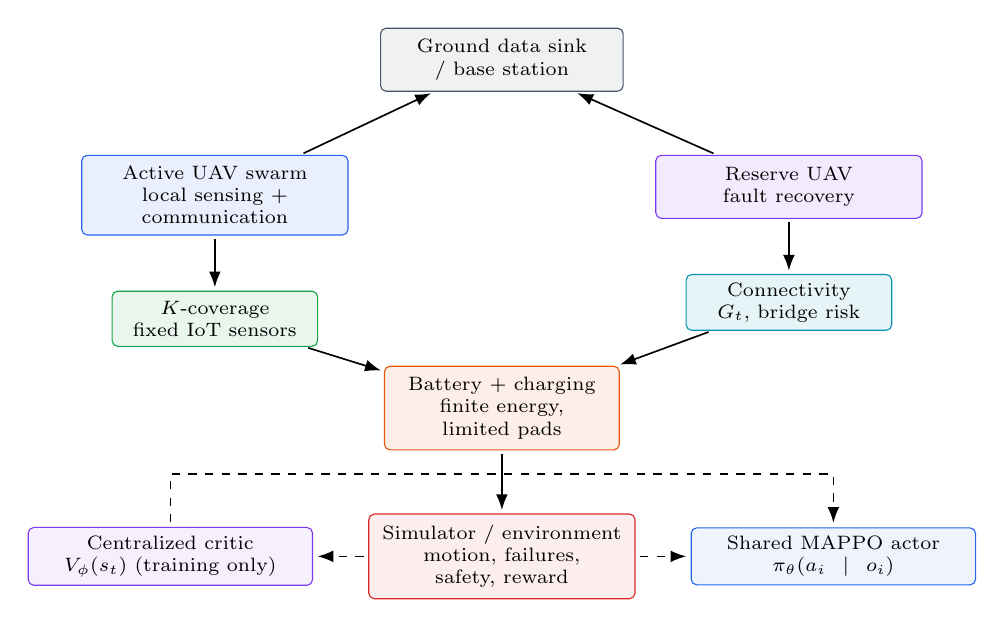
\begin{tikzpicture}[
node distance=6mm and 8mm,
box/.style={draw,rounded corners=2pt,align=center,font=\scriptsize,minimum height=8mm,inner sep=4pt},
small/.style={draw,rounded corners=2pt,align=center,font=\scriptsize,minimum height=7mm,inner sep=3pt},
arr/.style={-{Latex[length=2mm]},semithick,shorten >=1.2pt,shorten <=1.2pt},
darr/.style={-{Latex[length=2mm]},semithick,dashed,shorten >=1.6pt,shorten <=1.6pt}
]
\node[box,fill=uavgray!8,draw=uavgray,text width=28mm] (sink) {Ground data sink\\/ base station};
\node[box,fill=uavblue!10,draw=uavblue,text width=31mm,below left=8mm and 4mm of sink] (swarm) {Active UAV swarm\\local sensing + communication};
\node[box,fill=uavpurple!10,draw=uavpurple,text width=31mm,below right=8mm and 4mm of sink] (reserve) {Reserve UAV\\fault recovery};
\node[small,fill=uavgreen!10,draw=uavgreen,text width=24mm,below=7mm of swarm] (cov) {$K$-coverage\\fixed IoT sensors};
\node[small,fill=uavcyan!10,draw=uavcyan,text width=24mm,below=7mm of reserve] (conn) {Connectivity\\$G_t$, bridge risk};
\node[box,fill=uavorange!10,draw=uavorange,text width=27mm,below=7mm of $(cov)!0.5!(conn)$] (energy) {Battery + charging\\finite energy, limited pads};
\node[box,fill=uavred!8,draw=uavred,text width=31mm,below=8mm of energy] (env) {Simulator / environment\\motion, failures, safety, reward};
\node[small,fill=uavblue!8,draw=uavblue,text width=34mm,right=7mm of env] (actor) {Shared MAPPO actor\\$\pi_\theta(a_i\mid o_i)$};
\node[small,fill=uavpurple!8,draw=uavpurple,text width=34mm,left=7mm of env] (critic) {Centralized critic\\$V_\phi(s_t)$ (training only)};
\draw[arr] (swarm) -- (sink);
\draw[arr] (reserve) -- (sink);
\draw[arr] (swarm) -- (cov);
\draw[arr] (reserve) -- (conn);
\draw[arr] (cov) -- (energy);
\draw[arr] (conn) -- (energy);
\draw[arr] (energy) -- (env);
\draw[darr] (env) -- (actor);
\draw[darr] (env) -- (critic);
\coordinate (cfb) at ($(env.north)+(0,5mm)$);
\draw[darr] (critic.north) -- (critic.north |- cfb)
      -- (actor.north |- cfb) -- (actor.north);
\end{tikzpicture}%
}
\caption{Color-coded system architecture. Active UAVs provide sensor coverage and maintain a range-limited communication graph. The reserve UAV supports post-failure recovery. The shared MAPPO actor is deployed locally, while the centralized critic is used only during training.}
\label{fig:arch}
\end{figure}

For tractability, the UAVs fly at a common nominal altitude $z_0$, so the decision process operates in the horizontal plane while the altitude remains part of the physical state. Let $\mathbf p_i(t)=[x_i(t),y_i(t)]^\mathsf{T}$ denote the horizontal position of UAV $i$ and $\mathbf q_d=[x_d,y_d]^\mathsf{T}$ the position of sensor $d$.

\subsection{Dec-POMDP Formulation}
The cooperative control problem is represented as
\begin{equation}
\mathcal G=\langle N,\mathcal S,\{\mathcal A_i\},\{\mathcal O_i\},\mathcal T, R,\gamma\rangle,
\label{eq:decpomdp}
\end{equation}
where $\mathcal S$ is the global state space, $\mathcal A_i$ is the action space of UAV $i$, $\mathcal O_i$ is its local observation space, $\mathcal T$ is the transition model, $R$ is the shared reward, and $\gamma\in(0,1)$ is the discount factor. The training objective is
\begin{equation}
\max_{\pi}\;\mathbb E_{\pi}\left[\sum_{t=0}^{T-1}\gamma^t R_t\right].
\label{eq:objective}
\end{equation}

\subsection{Global State}
The state available to the centralized critic during training is
\begin{equation}
\mathbf s_t=\left\{(\mathbf p_i,\mathbf v_i,b_i,m_i,F_i)_{i=1}^{N},(\mathbf q_d)_{d=1}^{M},\mathbf Q_t\right\},
\label{eq:state}
\end{equation}
where $\mathcal{V}_t^{\mathrm{act}}=\{\,i\in\{1,\dots,N\}:F_i(t)=0\,\}$ is the set of active UAVs, from which any UAV with $F_i(t)=1$ is removed in all coverage, connectivity and energy sums. $\mathbf v_i$ is velocity, $b_i\in[0,1]$ is normalized battery level, $m_i\in\{\mathrm{serve},\mathrm{return},\mathrm{charge}\}$ is operating mode, $F_i\in\{0,1\}$ is the failure indicator, and $\mathbf Q_t\in\{0,1\}^{S}$ records charging-pad occupancy. A failed UAV is removed from the active set used in coverage and connectivity calculations.

\subsection{Local Observation}
At deployment, UAV $i$ uses only locally available information, plus two
broadcast quantities:
\begin{equation}
\mathbf o_i(t)=\left[\mathbf p_i,\mathbf v_i,b_i,\mathcal N_i,C_i^{\mathrm{local}},\rho_i,\tau_i^{\mathrm{return}},E_i^{\mathrm{pad}},\mathbf 1_i,\mathbf m_t\right].
\label{eq:obs}
\end{equation}
Here $\mathcal N_i$ is the set of nearby UAVs, $C_i^{\mathrm{local}}$ is the number of nearby sensors currently covered, $\rho_i$ is a locally computed bridge-risk estimate, $\tau_i^{\mathrm{return}}$ is the estimated time until the return threshold is reached, and $E_i^{\mathrm{pad}}$ is the estimated energy needed to reach a feasible charging pad. The last two terms are the agent's own identity $\mathbf 1_i\in\{0,1\}^{N}$ and a coarse coverage-map summary $\mathbf m_t\in[0,1]^{G\times G}$ of the share of under-covered sensors in each cell of the region, with $G=4$.

Two properties of this observation are not cosmetic, and both are load-bearing for the shared-parameter design of Section~\ref{sec:mappo}. The first is the identity. Parameter sharing is sound only when each agent's own observation identifies it, so that a shared network can still specialise~\cite{foerster2016}; the first version of $\mathbf o_i$ did not satisfy this condition, and the consequence was measurable rather than theoretical: in a symmetric deployment every agent received an almost identical input, the deterministic policy selected the same action for all of them, and the swarm translated as a rigid body without ever dispersing. The second is the map summary. Without it an agent knows how many sensors it covers but not which sensors are deficient, so nothing in $\mathbf o_i$ points towards the deficit and no gradient signal for deployment exists. We assume that the infrastructure which owns the charging pads also aggregates the IoT service reports and broadcasts the summary, which is a communication assumption rather than an oracle; the summary is fixed size, so the observation does not grow with the number of sensors. Section~\ref{sec:results} reports the measured effect of each term.

Unlike the idealized global articulation-point indicator sometimes used in analysis, $\rho_i$ is intended to be computable during execution from neighborhood exchange. The simulator may additionally compute the exact articulation-point indicator for evaluation and for the centralized critic. This distinction avoids assuming that an individual UAV can magically obtain the complete global topology.

\begin{table}[t]
\caption{Local observation variables available to each deployed UAV.}
\label{tab:obs}
\centering
\scriptsize
\renewcommand{\arraystretch}{1.06}
\begin{tabularx}{\columnwidth}{@{}L{1.3cm}L{1.7cm}Y@{}}
\toprule
Feature & Symbol & Meaning at decision time \\
\midrule
Position & $\mathbf p_i$ & Own horizontal location; altitude is fixed for the primary study. \\
Velocity & $\mathbf v_i$ & Current velocity for motion-limit awareness. \\
Battery & $b_i$ & Normalized remaining energy. \\
Neighbors & $\mathcal N_i$ & UAVs detected within $R_{\mathrm{comm}}$. \\
Coverage & $C_i^{\mathrm{local}}$ & Nearby sensors currently within coverage radius. \\
Bridge risk & $\rho_i$ & Local estimate of topology criticality. \\
Return urgency & $\tau_i^{\mathrm{return}}$ & Estimated time until the return-energy threshold. \\
Pad energy & $E_i^{\mathrm{pad}}$ & Estimated energy to the nearest feasible charging pad. \\
Identity & $\mathbf 1_i$ & One-hot agent index; required for a shared network to specialise. \\
Map summary & $\mathbf m_t$ & $G\times G$ share of under-covered sensors per cell (broadcast). \\
\bottomrule
\end{tabularx}
\end{table}

\subsection{Discrete Action Space and Motion}
Each active UAV selects one of six actions:
\begin{equation}
\mathcal A_i=\{\mathrm{Hover},+x,-x,+y,-y,\mathrm{Charge}\},\qquad |\mathcal A_i|=6.
\label{eq:actions}
\end{equation}
For movement actions,
\begin{equation}
\mathbf p_i(t+1)=\Pi_{\Omega}\left(\mathbf p_i(t)+\mathbf v_i(t)\Delta t\right),
\qquad \|\mathbf v_i(t)\|\le v_{\max},
\label{eq:motion}
\end{equation}

\begin{table}[t]
\caption{Discrete action semantics used by the MAPPO actor.}
\label{tab:actions}
\centering
\scriptsize
\renewcommand{\arraystretch}{1.05}
\begin{tabularx}{\columnwidth}{@{}L{1.35cm}Y@{}}
\toprule
Action & Effect \\
\midrule
Hover & Remain at the current position and continue serving covered sensors. \\
$+x$ / $-x$ & Move by one control step along the horizontal $x$ direction. \\
$+y$ / $-y$ & Move by one control step along the horizontal $y$ direction. \\
Charge & Request charging when inside a pad service region; pad selection is handled by the scheduler. \\
\bottomrule
\end{tabularx}
\end{table}
where $\Pi_{\Omega}$ projects into the permitted airspace. A charge request is feasible only when the UAV is inside a station neighborhood of a free pad. The RL layer does not select a pad as part of its action; pad choice is handled by the arbitration layer in Section~\ref{sec:charging}.

\subsection{Persistent $K$-Coverage}
\label{sec:coverage}
A UAV covers sensor $d$ in slot $t$ when
\begin{equation}
x_{id}(t)=\mathbb 1\!\left[\|\mathbf p_i(t)-\mathbf q_d\|_2\le R_{\mathrm{cov}}\right].
\label{eq:xid}
\end{equation}
The number of active UAVs covering sensor $d$ is
\begin{equation}
n_d(t)=\sum_{i\in\mathcal V_t^{\mathrm{act}}}x_{id}(t),
\label{eq:nd}
\end{equation}
and the instantaneous normalized coverage score is
\begin{equation}
C_t=\frac{1}{M}\sum_{d=1}^{M}\min\left(\frac{n_d(t)}{K},1\right).
\label{eq:Ct}
\end{equation}
The instantaneous under-coverage rate is
\begin{equation}
U_t=\frac{1}{M}\sum_{d=1}^{M}\mathbb 1[n_d(t)<K].
\label{eq:Ut}
\end{equation}
The primary service condition is $n_d(t)\ge K$ for all $d$ whenever the geometry and available fleet make it feasible.

\medskip
\noindent\textbf{Feasibility.} Persistent $K$-coverage is achievable only when the sensing radius is large enough for the available fleet. Comparing the area available for coverage with the area required gives a necessary condition: $N$ disks of radius $R_{\mathrm{cov}}$ supply $N\pi R_{\mathrm{cov}}^{2}$, while $K$-coverage of a region of area $A$ requires $KA$. Hence $R_{\mathrm{cov}} \ge \sqrt{KA/(\pi N)}$. Accounting for the $\delta = \pi/(2\sqrt{3}) \approx 0.907$ packing density of congruent disks gives the stricter form $R_{\mathrm{cov}} \ge \sqrt{KA/(\delta\pi N)}$. Substituting the parameters of Table~\ref{tab:parameters} ($A = 6400$ m$^2$, $M = 20$, $N = 5$, $K = 2$) yields $R_{\mathrm{cov}} \ge 28.5$ m by area counting and $30.0$ m after the packing correction, both satisfied by the chosen $R_{\mathrm{cov}} = 35$ m. The resulting surplus ratio $\sigma = N\pi R_{\mathrm{cov}}^{2}/(KA) = 1.50$ leaves margin for movement error and for a single-UAV failure, after which $\sigma = 1.20$ still exceeds one. The bound is necessary rather than sufficient, since it ignores coverage-disk overlap and the discreteness of the sensor layout; scenario S8 of Table~\ref{tab:scenarios} therefore sweeps $R_{\mathrm{cov}}$ directly to characterize the transition.

\begin{figure}[t]
\centering
% 3D schematic: oblique axonometric. UAVs fly at z_0 above the sensor plane.
% No \resizebox here: it would scale line widths and dash patterns too.
% The unit vectors below give the natural size (about 73 x 51 mm), which fits
% the 88.9 mm IEEE column width at true line widths and font sizes.
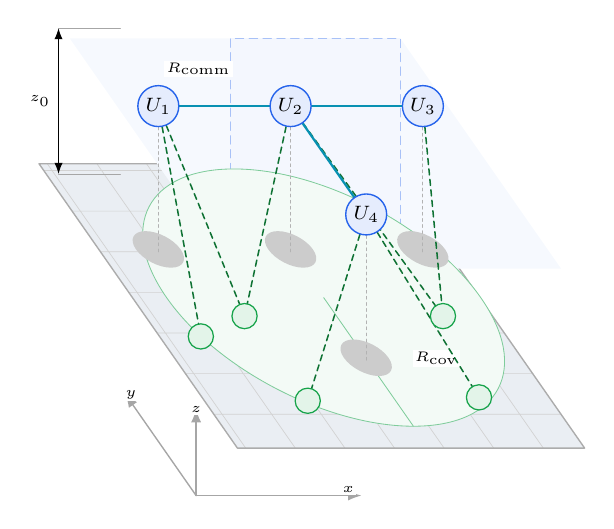
\begin{tikzpicture}[
pt/.style={circle,draw=uavblue,fill=uavblue!12,line width=0.5pt,
           minimum size=5.2mm,inner sep=0pt,font=\scriptsize},
sn/.style={circle,draw=uavgreen,fill=uavgreen!12,line width=0.45pt,
           minimum size=3.2mm,inner sep=0pt},
link/.style={draw=uavcyan,line width=0.8pt},
covlink/.style={draw=uavgreen!70!black,line width=0.55pt,
                dash pattern=on 2.2pt off 1.6pt},
drop/.style={draw=gray!60,line width=0.35pt,dash pattern=on 1pt off 1.2pt},
foot/.style={draw=uavgreen!55,line width=0.3pt,fill=uavgreen!5},
uavpl/.style={draw=uavblue!40,line width=0.4pt,
              dash pattern=on 3pt off 2pt,fill=uavblue!5},
guide/.style={draw=gray!70,line width=0.25pt},
axis/.style={-{Latex[length=1.7mm]},line width=0.5pt,draw=gray!70},
shadow/.style={fill=gray!40,draw=none},
ann/.style={font=\tiny,align=center,fill=white,inner sep=0.8pt},
x={(1.05cm,0cm)}, y={(-0.6cm,0.86cm)}, z={(0cm,1cm)},
line cap=round, line join=round
]
% ---- ground plane (fixed IoT sensors live on it) -------------------------
\begin{scope}[canvas is xy plane at z=0]
  \path[fill=gndgray] (-0.7,-2.9) rectangle (3.5,1.3);
  \draw[step=0.6,gray!35,line width=0.25pt] (-0.7,-2.9) grid (3.5,1.3);
  \draw[gray!65,line width=0.5pt] (-0.7,-2.9) rectangle (3.5,1.3);
\end{scope}
% ---- UAV operating plane at altitude z_0 (translucent, in front) ---------
\begin{scope}[canvas is xy plane at z=1.85]
  \path[fill=uavblue!4] (-0.5,-2.4) rectangle (3.5,1.0);
\end{scope}
\draw[uavpl] (-0.5,-2.4,1.85) rectangle (3.5,1.0,1.85);
% ---- horizontal coverage footprint, drawn on the ground -----------------
\begin{scope}[canvas is xy plane at z=0.02]
  \draw[foot] (1.6,-0.7) circle[radius=1.9];
  \draw[foot] (1.6,-0.7) -- (1.6,-2.6);
  \node[ann] at (2.45,-1.6) {$R_{\mathrm{cov}}$};
\end{scope}
% ---- ground shadows + vertical drop lines (depth cues) ------------------
\foreach \cx/\cy in {0/0,1.6/0,3.2/0,1.6/-1.6}{
  \begin{scope}[canvas is xy plane at z=0.03]
    \fill[shadow] (\cx,\cy) circle[radius=0.27];
  \end{scope}
  \draw[drop] (\cx,\cy,0) -- (\cx,\cy,1.85);
}
% ---- coverage links ------------------------------------------------------
\draw[covlink] (0,0,1.85)      -- (-0.2,-1.25,0);
\draw[covlink] (0,0,1.85)      -- (0.5,-0.95,0);
\draw[covlink] (1.6,0,1.85)    -- (0.5,-0.95,0);
\draw[covlink] (1.6,0,1.85)    -- (2.9,-0.95,0);
\draw[covlink] (3.2,0,1.85)    -- (2.9,-0.95,0);
\draw[covlink] (1.6,-1.6,1.85) -- (0.55,-2.2,0);
\draw[covlink] (1.6,-1.6,1.85) -- (2.65,-2.15,0);
% ---- sensors on the plane ------------------------------------------------
\foreach \cx/\cy in {-0.2/-1.25,0.5/-0.95,2.9/-0.95,0.55/-2.2,2.65/-2.15}
  \node[sn] at (\cx,\cy,0) {};
% ---- inter-UAV communication (all at equal altitude) ---------------------
\draw[link] (0,0,1.85) -- (1.6,0,1.85) -- (3.2,0,1.85);
\draw[link] (1.6,0,1.85) -- (1.6,-1.6,1.85);
\node[ann] at (0.8,0.55,1.85) {$R_{\mathrm{comm}}$};
% ---- UAVs (drawn last so they sit on top) -------------------------------
\node[pt] at (0,0,1.85)      {$U_1$};
\node[pt] at (1.6,0,1.85)    {$U_2$};
\node[pt] at (3.2,0,1.85)    {$U_3$};
\node[pt] at (1.6,-1.6,1.85) {$U_4$};
% ---- altitude dimension z_0 ---------------------------------------------
\draw[guide] (-0.55,1.15,0)    -- (0.2,1.15,0);
\draw[guide] (-0.55,1.15,1.85) -- (0.2,1.15,1.85);
\draw[{Latex[length=1.4mm]}-{Latex[length=1.4mm]},line width=0.4pt]
      (-0.55,1.15,0) -- (-0.55,1.15,1.85)
      node[ann,midway,left=2pt] {$z_0$};
% ---- projected x/y/z triad: unambiguous 3D frame ------------------------
\draw[axis] (-1.6,-3.6,0) -- (0.4,-3.6,0)   node[ann,pos=0.92,above] {$x$};
\draw[axis] (-1.6,-3.6,0) -- (-1.6,-2.1,0)   node[ann,pos=0.92,above] {$y$};
\draw[axis] (-1.6,-3.6,0) -- (-1.6,-3.6,1.1) node[ann,pos=0.92,above] {$z$};
\end{tikzpicture}
\caption{Coupling between coverage and connectivity in three dimensions. The shaded grid is the fixed sensor plane at $z=0$, and the translucent blue sheet is the UAV operating plane at the common nominal altitude $z_0$; the projected $x/y/z$ triad, the ground shadows and the dashed vertical drop lines fix the perspective. The green disc on the ground is the horizontal coverage footprint $R_{\mathrm{cov}}$ joined to the UAVs by dashed coverage links, whereas the cyan edges lying inside the UAV plane are inter-UAV communication links of range $R_{\mathrm{comm}}$. Removing a topologically critical UAV can reduce both service redundancy and network connectivity.}
\label{fig:coupling}
\end{figure}

\subsection{Feasibility Certificate for $K$-Coverage}
\label{sec:feasibility}

Before any policy is trained, the configuration must be shown to admit a feasible
solution. The report's original $N=5$, $K=2$, $R_{\mathrm{cov}}=35$\,m
configuration does \emph{not}: the four corner $K$-coverage discs are pairwise
disjoint because the corner separation $80$\,m exceeds $2R_{\mathrm{cov}}=70$\,m,
so covering the region requires $N\ge 4K=8$ (classical $k$-fold covering,
Kershner 1939). The area-surplus metric $\sigma=1.503$ does not rescue this:
an area ratio is not a covering bound.

\emph{Feasibility certificate (two bounds).}
\begin{itemize}
  \item \textbf{Region bound:} $N \ge 4K$ for a square of side $S$ with
    $S > 2R_{\mathrm{cov}}$. For $K=2$, $N\ge 8$.
  \item \textbf{Sensor-set bound:} $N \ge K\cdot |S|$ for a given sensor
    draw $S$. Over 30 random seeds this gives mean $4.4$, maximum $6$; so
    $N=5$ is feasible for \emph{most} random scenes but not universally.
\end{itemize}

\emph{Corrected, feasible deployments:} $N=8$, $K=2$, $R_{\mathrm{cov}}=35$\,m
(provably feasible) or $N=5$, $K=2$, $R_{\mathrm{cov}}=45$\,m ($R_{\mathrm{cov}}>42.5$\,m
required). All trained results in this paper use the former.

\emph{Achievability ceiling.} A teleporting placement oracle
(\texttt{analysis/feasibility.py}) upper-bounds any policy's coverage and
separates ``the policy is weak'' from ``the task is infeasible''. Policy
performance is reported as achieved divided by oracle.

\emph{Non-degenerate metrics.} The service-continuity metric
``fraction of time all sensors are $K$-covered \emph{and} the graph is
connected'' is identically zero on an infeasible configuration. It is retained
for comparison but supplemented by (i) a time-averaged coverage deficit
$\frac1T\sum_t(1-\overline{\mathrm{CK}}_t)$ and (ii) a maximum refresh time
(longest run of steps with any under-covered sensor).

\subsection{Connectivity Model}
The inter-UAV communication graph is
\begin{equation}
G_t=(V_t,E_t),\qquad E_t=\{(i,j):\|\mathbf p_i-\mathbf p_j\|_2\le R_{\mathrm{comm}}\}.
\label{eq:graph}
\end{equation}
The ground data sink is treated as an additional vertex with edges to every UAV within $R_{\mathrm{comm}}$; the swarm is connected when $G_t$ (including the sink) has one connected component. For analysis, the exact articulation-point indicator, where $G_t^{-i}$ denotes $G_t$ with vertex $i$ and its incident edges removed, is
\begin{equation}
\kappa_i(t)=\mathbb 1\left[G_t^{-i}\;\text{is disconnected}\right].
\label{eq:articulation}
\end{equation}
The average criticality is
\begin{equation}
\mathrm{Crit}_t=\frac{1}{|V_t^{\mathrm{act}}|}\sum_{i\in V_t^{\mathrm{act}}}\kappa_i(t).
\label{eq:crit}
\end{equation}
The exact graph quantity is used by the simulator for evaluation. The actor receives the local proxy $\rho_i$ rather than the full graph.

\subsection{Battery Model}
Let $B_i^{\max}$ be the battery capacity in joules and $E_i(t)=b_i(t)B_i^{\max}$ the remaining energy. The slot energy update is
\begin{equation}
E_i(t+1)=\mathrm{clip}\!\left(E_i(t)-P_i(t)\Delta t+P_{\mathrm{ch},i}(t)\Delta t,\;0,\;B_i^{\max}\right),
\label{eq:battery}
\end{equation}
where the action-dependent consumption is
\begin{equation}
\begin{split}
P_i(t)={}&P_{\mathrm{hover}}\,\mathbb 1[a_i=\mathrm{Hover}]\\
&+P_{\mathrm{move}}\,\mathbb 1[a_i\in\{+x,-x,+y,-y\}]+P_{\mathrm{comm}}.
\end{split}
\label{eq:power}
\end{equation}
The charge power is zero unless the UAV is physically docked and granted service at a pad. A return threshold is defined by
\begin{equation}
E_i^{\mathrm{req}}(t)=E_i^{\mathrm{pad}}(t)+E_i^{\mathrm{rejoin}}(t)+E^{\mathrm{reserve}},
\label{eq:ereq}
\end{equation}
and a return is mandatory when $E_i(t)\le E_i^{\mathrm{req}}(t)$.

Two properties of this model are easy to state and easy to implement incorrectly, and both were implemented incorrectly in the first version of the simulator, so both are pinned by tests. First, the return is a \emph{physical} transition and not a decision available to the policy: the simulator makes it, so that the reward, the metrics and the charging arbitration can all see it. If the simulator does not make it, then a learned policy has no way to express the return at all, the arbitration is never entered, and the reserve mechanism has nothing to recover --- the three mechanisms this paper proposes are then present in the model and absent from the experiment. Second, a UAV that is docked and charging has its rotors idle and draws only the avionics and communications baseline; if it is billed the hover power, the pack loses more energy to the rotors than the pad puts back, no UAV can ever recover, and the charging coordination is unusable. A UAV whose pack empties away from a pad is out of service: it can no longer fly, and it must not continue to count towards coverage or towards the connectivity graph.

\begin{figure}[t]
\centering
\resizebox{\columnwidth}{!}{%
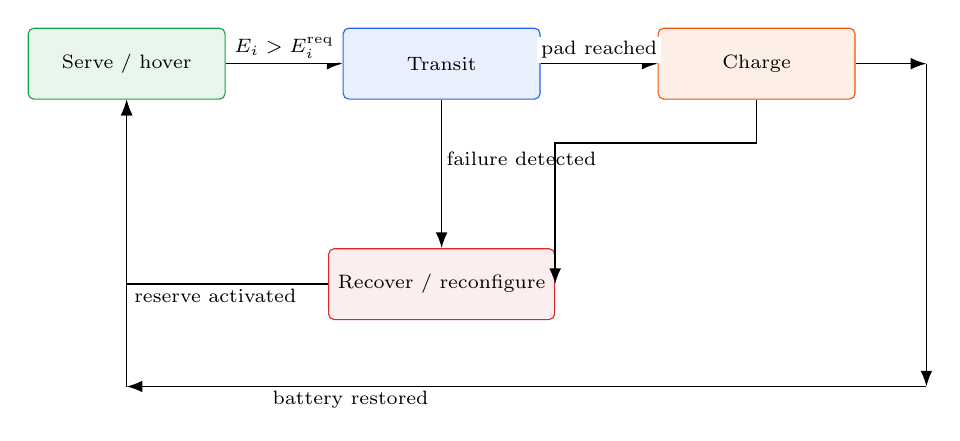
\begin{tikzpicture}[
state/.style={draw,rounded corners=2pt,minimum width=25mm,minimum height=9mm,align=center,font=\scriptsize},
arr/.style={-{Latex[length=2mm]},semithick},
lab/.style={font=\scriptsize,fill=white,inner sep=1.5pt}
]
\node[state,fill=uavgreen!10,draw=uavgreen]  (serve)   at (0,0)     {Serve / hover};
\node[state,fill=uavblue!10,draw=uavblue]    (transit) at (4.0,0)   {Transit};
\node[state,fill=uavorange!10,draw=uavorange] (charge) at (8.0,0)   {Charge};
\node[state,fill=uavred!8,draw=uavred]       (recover) at (4.0,-2.8) {Recover / reconfigure};
\draw[arr] (serve)  -- node[lab,above] {$E_i>E_i^{\mathrm{req}}$} (transit);
\draw[arr] (transit) -- node[lab,above] {pad reached} (charge);
\coordinate (rt) at ($(charge.east)+(0.9,0)$);
\coordinate (rb) at ($(rt)+(0,-4.1)$);
\draw[arr] (charge.east) -- (rt);
\draw[arr] (rt) -- (rb);
\draw[arr] (rb) -- node[lab,below,pos=0.72] {battery restored} (0,-4.1);
\draw[arr] (0,-4.1) -- (serve.south);
\draw[arr] (transit.south) -- node[lab,right,pos=0.40] {failure detected} (recover.north);
\draw[arr] (charge.south) -- ++(0,-0.55) -| (recover.east);
\draw[arr] (recover.west) -| node[lab,below,pos=0.28] {reserve activated} (serve.south);
\end{tikzpicture}%
}
\caption{Battery and failure state machine. Energy urgency triggers a return-to-charge transition; a detected failure transfers the mission to a recovery phase in which the reserve UAV can be activated when feasible.}
\label{fig:statemachine}
\end{figure}

\subsection{Charging Coordination}
\label{sec:charging}
Charging is a scarce resource. Let $y_{is}\in\{0,1\}$ denote whether UAV $i$ is assigned to pad $s$. For a charge request, define a local assignment cost
\begin{equation}
c_{is}=\alpha\tilde d_{is}+\beta\tilde q_s+\mu\tilde u_i,
\label{eq:chargingcost}
\end{equation}
where $\tilde d_{is}$ is normalized distance, $\tilde q_s$ is normalized queue length, and $\tilde u_i$ is normalized battery urgency. The arbitration layer solves
\begin{equation}
\begin{aligned}
\min_{\mathbf y}\quad &\sum_i\sum_s c_{is}y_{is}\\
\mathrm{s.t.}\quad &\sum_s y_{is}\le1,\ \forall i,\\
&\sum_i y_{is}\le1,\ \forall s,\\
&y_{is}\in\{0,1\}.
\end{aligned}
\label{eq:charging}
\end{equation}
Because only charge requests are handled, this is a small scheduling problem rather than a centralized trajectory controller. A Hungarian-style assignment implementation is sufficient for the expected fleet size.

\subsection{Safety Constraints}
\label{sec:safety_model}
The environment enforces
\begin{equation}
\begin{split}
&\|\mathbf v_i(t)\|\le v_{\max},\qquad \mathbf p_i(t)\in\Omega,\\
&\|\mathbf p_i(t)-\mathbf p_j(t)\|\ge d_{\mathrm{safe}},\ \forall i\ne j.
\end{split}
\label{eq:safety}
\end{equation}
An action is masked if it violates a locally predictable hard constraint such as workspace bounds, speed, minimum separation, or invalid charging. Connectivity is handled differently, and the distinction matters. The \emph{policy} is not assumed to predict connectivity from one-hop observations; it receives the local bridge-risk feature $\rho_i$ and the team reward penalises connectivity fragility, so nothing in the learning signal claims a global guarantee from purely local information. The \emph{simulator}, however, is a safety filter: it evaluates the prospective communication graph for every candidate action and masks any move that would leave the swarm unable to remain connected, including the $H$-step lookahead of Section~\ref{sec:algorithm}. The guarantee therefore comes from the safe-filter architecture, in which the filter has access to the true state, and not from the policy's own foresight. The distinction is the standard one between learning which action to take and being told which actions are admissible.

\subsection{Failure and Recovery}
A failure event changes $F_i$ from $0$ to $1$ at the detection instant $t_f$. One reserve UAV is maintained with sufficient energy for deployment when feasible. After a detected failure, the reserve is activated and the active UAVs continue using their decentralized policies. The recovery time is defined as
\begin{equation}
\tau_f=\inf\left\{\tau\ge0:\ n_d(t_f+\tau)\ge K,\ \forall d\right\},
\label{eq:recovery}
\end{equation}
when recovery is achieved before the evaluation horizon. If recovery is impossible under the available fleet, the event is reported as an unrecovered failure rather than assigning an artificial recovery time.

A second mode of loss of an active UAV is exhaustion rather than failure: a UAV whose pack empties while it is away from a charging pad can neither fly nor serve, and it is removed from the active set. Such a UAV is out of service rather than failed, and the same reserve mechanism can re-seat it. This distinction is not cosmetic. If an exhausted UAV were left in the active set it would continue to count towards coverage and towards the connectivity graph while being unable to do either, and the reported coverage would be optimistic by exactly the number of sensors such a UAV was covering.

A recovery-time guarantee is therefore conditional: the reserve mechanism can reduce the time required for reconfiguration, but it cannot mathematically guarantee restoration for arbitrary sensor layouts, fleet sizes, or multiple simultaneous failures. This distinction is important for a realistic system model.

\subsection{Primary Objective and Reward Function}
The project formulation adopts a ``service first, efficiency second'' objective. The primary quantity is persistent service loss, represented by the fraction of IoT sensors that are below the required redundancy level. Let
\begin{equation}
J_{\mathrm{out}}(\pi)=\mathbb E_{\pi}\left[\sum_{t=0}^{T-1}\gamma^t U_t\right],
\label{eq:primaryobjective}
\end{equation}
where $U_t$ is the under-coverage rate in \eqref{eq:Ut}. The control policy therefore prioritizes minimizing long-horizon service loss rather than minimizing energy alone.

The corresponding multi-objective optimization is
\begin{equation}
\begin{aligned}
\min_{\pi}\quad &J_{\mathrm{out}}(\pi)+\lambda_EJ_E(\pi)+\lambda_DJ_D(\pi)\\
&+\lambda_WJ_W(\pi)+\lambda_RJ_R(\pi)+\lambda_CJ_C(\pi),
\end{aligned}
\label{eq:multiobjective}
\end{equation}
subject to the physical constraints in Section~\ref{sec:safety_model}. The secondary terms represent energy expenditure, degraded-service time, unnecessary movement, recovery delay, and topology criticality, respectively.

For reinforcement learning, the constrained objective is converted into a shared team reward:
\begin{equation}
\begin{aligned}
r_t=-\big(&\lambda_O U_t+\lambda_E E_t^{\mathrm{cons}}+
          \lambda_D D_t^{\mathrm{deg}}+\lambda_W W_t^{\mathrm{mov}}\\
&+\lambda_R R_t^{\mathrm{rec}}+\lambda_C\mathrm{Crit}_t\big).
\end{aligned}
\label{eq:reward}
\end{equation}
Since the learner maximises expected return while the control objective of \eqref{eq:multiobjective} is a minimisation, the team reward of \eqref{eq:reward} is the negated weighted cost, and the two are equivalent up to sign. Table~\ref{tab:reward} defines each term and gives the initial weights used in this work. The weight $\lambda_O$ is chosen to dominate the secondary efficiency terms, so that the learned controller does not sacrifice persistent service merely to reduce energy consumption or flight distance. The individual objective components remain separate evaluation metrics rather than being hidden inside a single final score.

\begin{table}[t]
\caption{Team reward terms and their initial weights.}
\label{tab:reward}
\centering
\scriptsize
\renewcommand{\arraystretch}{1.06}
\begin{tabularx}{\columnwidth}{@{}L{1.45cm}L{2.95cm}Y@{}}
\toprule
Term & Definition & Weight \\
\midrule
$U_t$ & Under-coverage rate, \eqref{eq:Ut} & $\lambda_O = 1.00$ \\
$E_t^{\mathrm{cons}}$ & $\sum_i\Delta E_i(t)\,/\,(N B^{\max})$ & $\lambda_E = 0.10$ \\
$D_t^{\mathrm{deg}}$ & 1 if any service requirement is violated & $\lambda_D = 2.00$ \\
$W_t^{\mathrm{mov}}$ & distance flown $/$ distance that changed coverage & $\lambda_W = 0.05$ \\
$R_t^{\mathrm{rec}}$ & normalized recovery delay during recovery & $\lambda_R = 0.30$ \\
$\mathrm{Crit}_t$ & Articulation-point average, \eqref{eq:crit} & $\lambda_C = 0.50$ \\
\bottomrule
\end{tabularx}
\end{table}

All six quantities are dimensionless and lie in $[0,1]$, so the weights are directly comparable; $U_t$ and $\mathrm{Crit}_t$ are already normalized in \eqref{eq:Ut} and \eqref{eq:crit}. The values are initial settings to be tuned on a validation set. The implemented values raise $\lambda_D$ above $\lambda_O$ so that a degraded-service step is penalised more heavily than a merely under-covered one; $\lambda_C$ is likewise raised so that connectivity loss is not drowned out by coverage. The ordering on which the formulation depends is $\lambda_D \ge \lambda_O \ge \lambda_C \ge \lambda_R > \lambda_E \ge \lambda_W$.

\begin{table}[t]
\caption{Hard constraints versus learned trade-offs.}
\label{tab:hardsoft}
\centering
\scriptsize
\renewcommand{\arraystretch}{1.06}
\begin{tabularx}{\columnwidth}{@{}L{1.38cm}L{2.05cm}Y@{}}
\toprule
Constraint & Mathematical form & Enforcement / evaluation \\
\midrule
Speed & $\|\mathbf v_i\|\le v_{\max}$ & Built into the action model and feasibility mask. \\
Workspace & $\mathbf p_i\in\Omega$ & Action mask prevents leaving the allowed region. \\
Separation & $\|\mathbf p_i-\mathbf p_j\|\ge d_{\mathrm{safe}}$ & Action mask prevents predicted collisions. \\
Battery reachability & $E_i\ge E_i^{\mathrm{req}}$ before departure & Prevents continuation when reaching a feasible charger is unsafe. \\
Charging capacity & At most one UAV per pad & Explicit pad assignment / scheduler. \\
$K$-coverage & $n_d(t)\ge K$ & Collective service objective and evaluation metric; not guaranteed by a single-agent mask. \\
Connectivity & $G_t$ connected & Topology-aware reward and connectivity metric. \\
Recovery & $\tau_f\le\tau_{\max}$ when feasible & Measured scenario requirement, not an unconditional guarantee. \\
\bottomrule
\end{tabularx}
\end{table}

\subsection{Parameter Settings and Scope}
Table~\ref{tab:parameters} gives the initial simulation configuration derived from the project layout. These are implementation parameters for the proposed simulator rather than experimentally calibrated real-flight values.

\begin{table}[t]
\caption{Initial simulation parameters.}
\label{tab:parameters}
\centering
\scriptsize
\begin{tabular}{@{}lll@{}}
\toprule
Parameter & Symbol & Value \\
\midrule
Active UAVs & $N$ & 8 (feasible; was 5, provably infeasible for $K=2$) \\
Reserve UAVs & $N_R$ & 1 \\
IoT sensors & $M$ & 20 \\
Operating region & $\Omega$ & $80\times80$ m$^2$ \\
Coverage radius & $R_{\mathrm{cov}}$ & 35 m \\
Communication radius & $R_{\mathrm{comm}}$ & 40 m \\
Nominal altitude & $z_0$ & 50 m \\
Coverage target & $K$ & 2 \\
Control interval & $\Delta t$ & 0.2 s \\
Maximum speed & $v_{\max}$ & 5 m/s \\
Safety distance & $d_{\mathrm{safe}}$ & 5 m \\
Battery capacity & $B^{\max}$ & 30,000 J \\
Hover power & $P_{\mathrm{hover}}$ & 50 W \\
Move power & $P_{\mathrm{move}}$ & 75 W \\
Avionics and comms power & $P_{\mathrm{elec}}$ & 5 W \\
RF transmit power & $P_{\mathrm{tx}}$ & 0.5 W \\
Charge increment & -- & 0.0002 battery fraction/step \\
Episode length & $T$ & 2000 steps (400\,s) \\
Initial deployment & -- & connected cluster in one corner \\
Map summary grid & $G$ & $4\times4$ cells \\
\bottomrule
\end{tabular}
\end{table}

The control interval is chosen so that the relative displacement between two consecutive steps, $2 v_{\max}\Delta t = 2$ m, is smaller than the safety distance $d_{\mathrm{safe}} = 5$ m; a coarser step would allow a closing pair to cross the separation constraint between two samples. The charge increment is quoted per step and is therefore scaled with $\Delta t$. The resulting charge time is shorter than a real constant-current pack of this capacity would require, because a real pack would not complete a full charge within a tractable episode; this is stated as a modelling assumption rather than a physical prediction, and it means the cost of charging contention in \eqref{tab:metrics} is a lower bound. The nominal altitude is consistent with the coverage radius: a $74^\circ$ downward sensor at 50 m yields a footprint half-width of 37 m. The two power entries are distinct: $P_{\mathrm{elec}}$ is the total avionics and communications budget, whereas $P_{\mathrm{tx}}$ is the radiated transmit power, which is bounded by the 1 W ceiling of IEEE 802.11 and is two orders of magnitude below the avionics budget. The chosen $v_{\max}=5$~m/s is conservative but not arbitrary: Luna et al.~\cite{luna2022} report a real three-UAV coverage mission flown at 5~m/s cruise and 20~m altitude, and Datsko et al.~\cite{datsko2024} measure the energy-optimal multirotor cruise speed at 8.39~m/s.

\paragraph{The initial deployment and the episode length are experimental choices,
and they are stated as such.}
Two parameters of Table~\ref{tab:parameters} deserve an explicit justification, because the results are sensitive to both and a reader should be able to see why they were chosen.

\emph{Initial deployment.} The swarm starts as a connected cluster in one corner of the region, not as a deployed formation. The reason is measurable: a centred ring deployment already covers 17 of the 20 sensors at $t=0$, so every controller --- including one that never moves --- scores $CK=0.850$, the achievable range is roughly $[0.85,1.0]$, and the comparison cannot separate the methods. The clustered deployment is connected at $t=0$, so the connectivity invariant remains checkable from the first step, but it covers only 3 of the 20 sensors, so the controller has to deploy across the field while holding $K=2$ redundancy. This is the standard arrangement for a persistent-coverage benchmark, and the pre-deployed arrangement is retained as scenario S9 so that the sensitivity is reported rather than hidden.

\emph{Episode length.} The episode is 2000 control steps, i.e.\ 400\,s of flight. At the 400-step episodes used in an earlier revision the pack never depleted: the swarm spent at most 13\% of a 600\,s pack, so the return-to-charge transition never fired, the charging arbitration was never entered, the reserve UAV had nothing to recover, and the three mechanisms the paper proposes were never exercised. A sweep over the candidate configurations (\texttt{analysis/energy\_regime.py}) shows that at 2000 steps the energy constraint binds --- 283 return-to-charge transitions and 0.7 stranded UAVs per episode under the Reactive heuristic --- while the mission remains achievable. The report's 10\,000-step target is a different question, and the results here are explicitly 400\,s results.

Within scope are spatial $K$-coverage, range-limited UAV connectivity, battery depletion, charging contention, single-UAV failure recovery, collision avoidance, and decentralized motion-policy execution. The primary model intentionally abstracts stochastic PHY-layer fading, detailed aerodynamic dynamics, obstacles, wind, battery aging, GPS denial, sensor failures, and multiple simultaneous UAV failures. These can be introduced as subsequent stress-test layers after the base control problem is validated.

\paragraph{Consistency of the physical parameters.}
The audit of Section~\ref{sec:validation} also records the derived physical
quantities, so that the modelling choices are explicit rather than implicit.
The endurance implied by $B^{\max}$ and $P_{\mathrm{hover}}$ is
$30{,}000/50=600$~s (10~min); the power ratio $P_{\mathrm{move}}/P_{\mathrm{hover}}=1.5$ is conservative against the 1.09 measured by Datsko et al.~\cite{datsko2024} for energy-optimal multirotor flight; and the charge increment of $2\times10^{-4}$ of the pack per step corresponds to a full charge in 1000~s, i.e.\ a 3.6~C rate, which is above the $\le 1$~C of hobby LiPo and is therefore an explicit modelling assumption rather than a physical prediction. Two further observations matter for the interpretation of the results. First, the separation constraint is enforced at the sample rate: two UAVs closing head-on at $2v_{\max}$ have a braking distance of $v_{\mathrm{close}}^{2}/(2a)=25$~m at $a=2$~m/s$^2$, five times $d_{\mathrm{safe}}$, so the mask guarantees sample-time separation and not braking. Second, at $N=8$ on an $80\times80$~m field the inter-UAV graph is not always dense: measured over a 2000-step flight in the deployed regime, the mean node degree is $4.01$ of a possible $7$, the graph is complete in only $12\%$ of steps, and nodes of degree $\le 1$ --- whose removal would isolate part of the swarm --- occur in a substantial fraction of UAV-steps. Connectivity is therefore a live constraint throughout the mission and not only after a failure, which is what makes the $H$-step mask and the reserve mechanism load-bearing rather than decorative. All four quantities are reported rather than silently adjusted, because changing them would change the measured results and the results are the claim.


\begin{figure*}[t]
\centering
\resizebox{0.93\textwidth}{!}{%
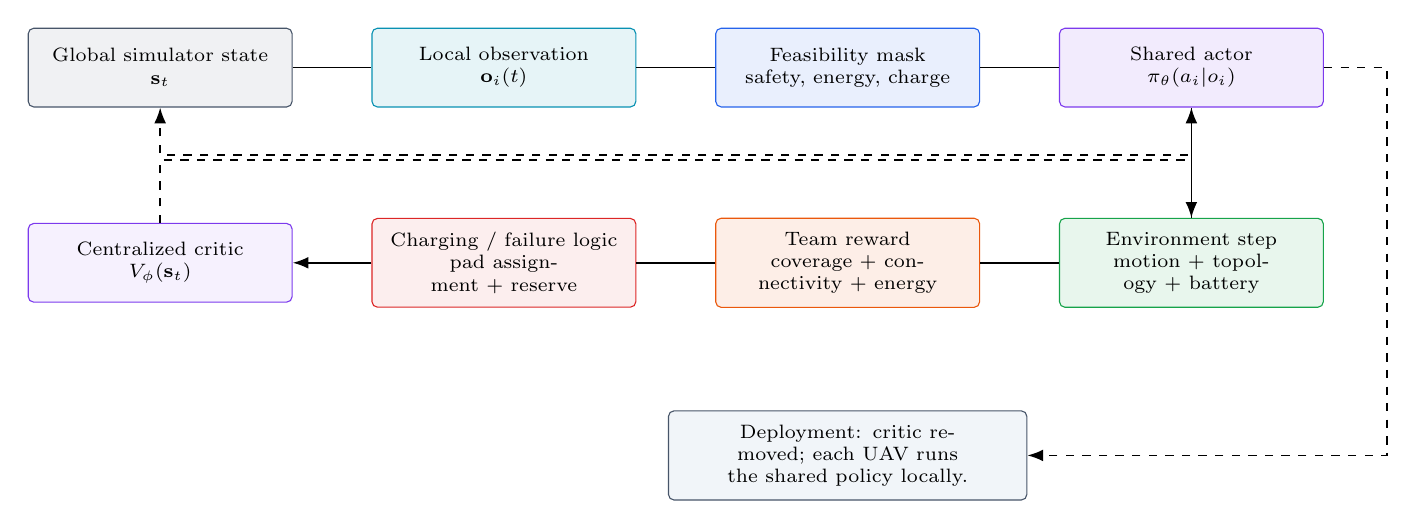
\begin{tikzpicture}[
node distance=7mm and 10mm,
box/.style={draw,rounded corners=2pt,align=center,font=\scriptsize,minimum height=10mm,inner sep=5pt},
arr/.style={-{Latex[length=2mm]},semithick},
darr/.style={-{Latex[length=2mm]},semithick,dashed}
]
\node[box,fill=uavgray!8,draw=uavgray,text width=30mm] (state) {Global simulator state\\$\mathbf s_t$};
\node[box,fill=uavcyan!10,draw=uavcyan,text width=30mm,right=of state] (obs) {Local observation\\$\mathbf o_i(t)$};
\node[box,fill=uavblue!10,draw=uavblue,text width=30mm,right=of obs] (mask) {Feasibility mask\\safety, energy, charge};
\node[box,fill=uavpurple!10,draw=uavpurple,text width=30mm,right=of mask] (actor) {Shared actor\\$\pi_\theta(a_i|o_i)$};
\node[box,fill=uavgreen!10,draw=uavgreen,text width=30mm,below=14mm of actor] (env) {Environment step\\motion + topology + battery};
\node[box,fill=uavorange!10,draw=uavorange,text width=30mm,left=of env] (reward) {Team reward\\coverage + connectivity + energy};
\node[box,fill=uavred!8,draw=uavred,text width=30mm,left=of reward] (failure) {Charging / failure logic\\pad assignment + reserve};
\node[box,fill=uavpurple!7,draw=uavpurple,text width=30mm,left=of failure] (critic) {Centralized critic\\$V_\phi(\mathbf s_t)$};
\draw[arr] (state)--(obs)--(mask)--(actor)--(env);
\draw[arr] (env)--(reward)--(failure)--(critic);
\draw[darr] (critic.north) |- ++(0,8mm) -| (actor.south);
\draw[darr] (env.north) |- ++(0,8mm) -| (state.south);
\node[box,fill=uavlight,draw=uavgray,text width=42mm,below=13mm of reward] (deploy) {Deployment: critic removed; each UAV runs the shared policy locally.};
\coordinate (adr) at ($(actor.east)+(8mm,0)$);
\coordinate (ddr) at (adr |- deploy.east);
\draw[darr] (actor.east) -- (adr) -- (ddr) -- (deploy.east);
\end{tikzpicture}%
}
\caption{MAPPO training and deployment pipeline. Solid arrows represent the environment/control loop. Dashed arrows denote training-only critic feedback and transfer of the learned actor to decentralized execution.}
\label{fig:pipeline}
\end{figure*}

\section{Proposed ML Algorithm}
\label{sec:algorithm}

\subsection{CTDE MAPPO}
\label{sec:mappo}
The proposed algorithm uses parameter-shared MAPPO. During training, the centralized critic observes $\mathbf s_t$ while every actor uses $\mathbf o_i(t)$. During deployment, the critic is removed and each UAV evaluates the same shared policy:
\begin{equation}
a_i(t)\sim\pi_{\theta}\left(a_i\mid\mathbf o_i(t)\right).
\label{eq:policy}
\end{equation}
Parameter sharing is appropriate when (i) the environment is equivariant to agent permutations---identical observation and action spaces and identical transition/reward structure---and (ii) each agent's own observation identifies it, so a shared network can still specialise (Foerster et al. \cite{foerster2016}). Condition (ii) is what the identity term $\mathbf 1_i$ of Eq.~\eqref{eq:obs} exists to satisfy, and it is worth being explicit that the first version of $\mathbf o_i$ did not satisfy it: the observation distinguished agents only through their individual position, battery and mode, which in a symmetric deployment are nearly identical across the swarm. The measured consequence was that the deterministic policy chose the same action for every UAV and the swarm moved as a rigid body, so the shared-parameter claim could not be sustained on the evidence. We therefore treat $\mathbf 1_i$ as part of the model rather than as an implementation detail, and Section~\ref{sec:results} reports the controlled comparison. The known limitation (Fu et al. \cite{fu2022}, Theorem 4.2) is that a shared policy provably cannot learn an optimal policy for non-symmetric tasks such as the XOR game; this does not apply here because the swarm is homogeneous. If grounded or docked UAVs with heterogeneous roles are introduced, parameters must not be shared.

For a collected rollout, the temporal-difference residual is
\begin{equation}
\delta_t=R_t+\gamma V_{\phi}(\mathbf s_{t+1})-V_{\phi}(\mathbf s_t),
\label{eq:tdres}
\end{equation}
and the generalized advantage estimate (GAE) is
\begin{equation}
\widehat A_t=\sum_{l=0}^{T-t-1}(\gamma\lambda)^l\delta_{t+l}.
\label{eq:gae}
\end{equation}
A fixed-length rollout ends either in a genuine terminal state or in a time-limit truncation, and the two must not be conflated. At a truncation boundary the last state is not absorbing, so the advantage recursion must cut without treating the state as terminal; the correct treatment is to bootstrap the temporal-difference residual from $V(\mathbf s_{T})$ rather than from zero~\cite{pardo2018}. Conflating the two injects a systematic downward bias into the advantage estimates. This is not a hypothetical concern for this work: the simulator initially reported the end of the mission time limit through the same flag it used for a genuine dead end, so every episode boundary was bootstrapped from zero and every value target was biased downward. The simulator now reports termination and truncation separately --- the mission time limit is a truncation, and only the loss of every UAV is a terminal state --- and the rollout consults that flag rather than inferring termination from the episode-end flag. The distinction is pinned by unit tests, one of which asserts that a time-limit episode is reported as a truncation and not as a termination, and another that asserts the rollout reads the environment's flag rather than re-deriving it.
The probability ratio is
\begin{equation}
r_t(\theta)=\frac{\pi_\theta(a_t\mid o_t)}{\pi_{\theta_{\mathrm{old}}}(a_t\mid o_t)}.
\end{equation}
The clipped PPO objective is
\begin{equation}
\begin{aligned}
L^{\mathrm{actor}}(\theta)=-\mathbb E_t\big[\min(&r_t\widehat A_t,\\
&\mathrm{clip}(r_t,1-\epsilon,1+\epsilon)\widehat A_t)\big].
\end{aligned}
\label{eq:actorloss}
\end{equation}
The critic is trained with the clipped MAPPO form (Yu et al. 2022, Appendix A):
\begin{equation}
L^{\mathrm{critic}}(\phi)=\mathbb E_t\!\left[\max\!\left((V_\phi(\mathbf s_t)-\widehat R_t)^2,\;
(\mathrm{clip}(V_\phi(\mathbf s_t),V_{\phi_{\mathrm{old}}}(\mathbf s_t)-\epsilon,
V_{\phi_{\mathrm{old}}}(\mathbf s_t)+\epsilon)-\widehat R_t)^2\right)\right],
\label{eq:criticloss}
\end{equation}
where $\widehat R_t=\widehat A_t+V_{\phi_{\mathrm{old}}}(\mathbf s_t)$ is the TD($\lambda$) lambda-return, computed once per rollout and treated as a constant (gradients are not propagated through it). The report matches the reference implementation (\texttt{r\_mappo.py}), which computes $\mathrm{gae}+\mathrm{value\_preds}$ rather than the Monte-Carlo return-to-go described in MAPPO's Appendix A prose.

\paragraph{Value normalisation, and the scale trap inside it.}
Value normalisation is one of the components the MAPPA/MAPPO literature identifies as load-bearing, and it was missing from the implementation while the earlier revision of this report asserted it. It is now present, and the details matter. The critic is trained to predict the returns in a \emph{normalised} space defined by running statistics of the return distribution, maintained as an exponential moving average with $\beta=0.99$:
\begin{equation}
\widehat R_t^{\mathrm{norm}}=\frac{\widehat R_t-\mu}{\sigma+\epsilon},
\label{eq:valuenorm}
\end{equation}
where $\mu$ and $\sigma$ are updated from the current rollout's returns. The consequence is easy to get wrong: the critic's \emph{raw} output is then the normalised value, so the temporal-difference residual of Eq.~\eqref{eq:tdres}, the advantage recursion of Eq.~\eqref{eq:gae}, and the bootstrap at a truncation boundary must all \emph{un-normalise} it before use, as $V(\mathbf s)=\sigma\,\hat V_\phi(\mathbf s)+\mu$. Reading the raw critic output at any of those three points is a silent scale error in the advantage estimates: the training loss still decreases, the entropy still falls, and the policy is simply trained against the wrong signal. The implementation therefore exposes a single accessor for the value and the test suite asserts that the rollout uses it rather than the raw output; a second test asserts that the value-clipping auxiliary term compares two quantities in the same space, since the recorded old value is in the original scale.

The advantage is normalised as well, by the mean and standard deviation of the batch. We also implemented a per-agent variant, in which each agent's advantages are normalised over its own history rather than over the pooled batch, and we report the measurement in Section~\ref{sec:results}: with a shared team reward every agent's advantage sequence is nearly identical, so the per-agent normalisation is close to a rescaling and does not change the credit assignment, which is the limitation of shared team rewards rather than a normalisation choice.

\subsection{Action Feasibility Mask}
Before the sampled action is executed, the simulator evaluates the predicted next position and applies the following checks: workspace bounds, maximum speed, minimum UAV separation, charge validity, and connectivity-preservation constraints. If a candidate movement would disconnect the communication graph, it is masked in normal operation. During an active recovery event, the connectivity rule remains a hard constraint unless the simulator enters a predefined recovery mode in which temporary reconnection is required by the recovery objective.

This separation between policy learning and hard feasibility is important. The neural network learns how to trade off several feasible actions, while the safety layer prevents the network from selecting actions that violate non-negotiable physical constraints.

The masking is applied at the logit level, before the softmax, so that the policy that is sampled from, the importance ratio that is computed against, and the entropy bonus that is regularised are all the same masked distribution. This is the mechanism that Huang and Onta~$n$~\cite{huang2022} show to correspond to a valid policy-gradient update rather than a biased surrogate: masking is implemented as a state-dependent differentiable transformation of the action-probability distribution, which is exactly what setting the masked logits to $-\infty$ before the softmax does. We note the limit of that result, which was stated explicitly in the same work and is repeated in the UAV action-masking literature~\cite{rizvi2025}: the validity argument is formulated for a single policy, and extending it to a centralized critic with heterogeneous per-agent masks requires the critic's training distribution to be consistent with the induced joint-action support. We therefore apply the identical mask to the rollout distribution, the stored log-probabilities and the update, and we verify this by construction in the test suite rather than by assumption.

\subsection{Failure-Aware Execution}
When a failure event is detected, the environment removes the failed UAV from the active graph, activates the reserve UAV if the reserve is available, and updates the local observations. The reserve UAV uses the same shared actor after insertion into the mission. The other UAVs also re-evaluate their local bridge-risk and coverage information. No prediction of the failure event is required; the controller reacts to the observed state change.

\begin{algorithm}[t]
\caption{MAPPO training algorithm}
\label{alg:training}
\begin{algorithmic}[1]
\STATE Initialize shared actor $\pi_\theta$ and centralized critic $V_\phi$.
\FOR{each training episode}
    \STATE Reset UAV positions, batteries, sensors, charging pads, and failure schedule.
    \FOR{$t=0,\ldots,T-1$}
        \STATE Construct global state $\mathbf s_t$ and each local observation $\mathbf o_i(t)$.
        \FOR{each active UAV $i$}
            \STATE Construct the feasible-action mask from Section~\ref{sec:system}.
            \STATE Sample $a_i(t)\sim\pi_\theta(\cdot\mid\mathbf o_i(t))$ over feasible actions.
        \ENDFOR
        \STATE Apply UAV actions and update positions.
        \STATE Recompute coverage and communication graph.
        \STATE Update battery states using \eqref{eq:battery}.
        \IF{one or more UAVs request charging}
            \STATE Solve the charging assignment in \eqref{eq:charging}.
        \ENDIF
        \IF{a UAV failure is detected}
            \STATE Activate the reserve UAV if feasible and update active-agent states.
        \ENDIF
        \STATE Compute $R_t$ from \eqref{eq:reward}; store rollout transition data.
    \ENDFOR
    \STATE Compute GAE advantages from \eqref{eq:gae}.
    \STATE Update $\theta$ with the clipped PPO objective.
    \STATE Update $\phi$ with the critic loss.
\ENDFOR
\RETURN Shared decentralized actor $\pi_\theta$.
\end{algorithmic}
\end{algorithm}

\subsection{Mapping from Model to Algorithm}
The algorithm is deliberately aligned with the system model. Sensor positions produce the coverage quantities in \eqref{eq:xid}--\eqref{eq:Ut}; neighboring UAV positions produce the communication graph in \eqref{eq:graph}; battery and action information produce the energy state in \eqref{eq:battery}; charging requests enter the assignment problem in \eqref{eq:charging}; and failure indicators activate the recovery process in \eqref{eq:recovery}. Thus, every actor input corresponds to an explicitly defined state quantity and every learned action has a defined environmental effect.

\subsection{Training and Generalization Protocol}
Training episodes should randomize sensor layouts, initial UAV positions, initial battery levels, charging-pad locations within the allowed region, and failure times. A simple curriculum can be used: first train under no failures, then introduce single failures, and finally introduce simultaneous charging contention and near-disconnection scenarios. The final model should be evaluated on held-out random seeds and scenario configurations not used for parameter tuning.

A practical implementation can use a multilayer perceptron for the shared actor and centralized critic with normalized numerical features and masked action logits. If fixed-length neighbor features are insufficient, a permutation-invariant pooling operation or a small attention encoder can be added without changing the underlying Dec-POMDP formulation. A recurrent policy should be introduced only if experiments show that instantaneous observations do not provide sufficient temporal information.


\subsection{Training Hyperparameters}
The initial training configuration follows the values in the project presentation. These values are starting points for the implementation and can be tuned on a validation set without changing the system formulation.

\begin{table}[t]
\caption{Initial MAPPO training configuration.}
\label{tab:hyper}
\centering
\scriptsize
\renewcommand{\arraystretch}{1.05}
\begin{tabular}{@{}lll@{}}
\toprule
Parameter & Symbol & Initial value \\
\midrule
Active UAVs & $N$ & 8 \\
IoT sensors & $M$ & 20 \\
Discount factor & $\gamma$ & 0.99 \\
PPO clipping & $\epsilon$ & 0.20 \\
GAE parameter & $\lambda$ & 0.95 \\
Control interval & $\Delta t$ & 0.2 s \\
\bottomrule
\end{tabular}
\end{table}

\subsection{Implementation Plan}
The implementation follows the three-stage validation strategy presented in the project plan. The objective is to validate the swarm-control logic before introducing detailed wireless-channel complexity.

\begin{figure}[t]
\centering
\resizebox{\columnwidth}{!}{%
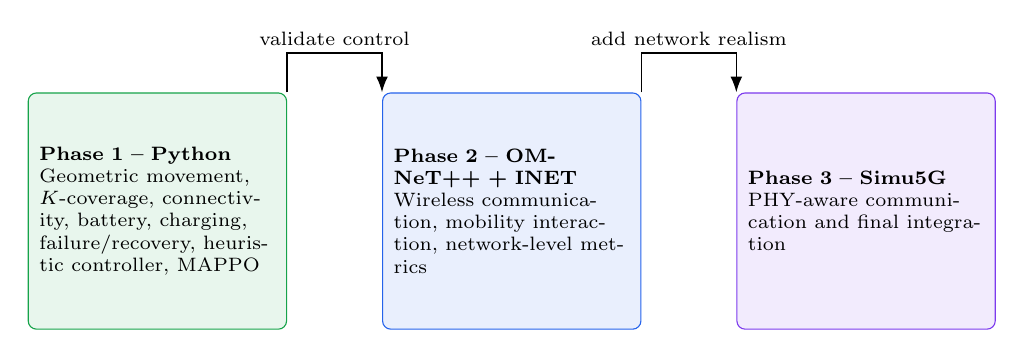
\begin{tikzpicture}[
phase/.style={draw,rounded corners=3pt,align=left,text width=30mm,minimum height=30mm,font=\scriptsize,inner sep=4pt},
arr/.style={-{Latex[length=2mm]},semithick},
lab/.style={font=\scriptsize,fill=white,inner sep=1.5pt}
]
\node[phase,anchor=north,fill=uavgreen!10,draw=uavgreen] (p1) at (0,0) {\textbf{Phase 1 -- Python}\\Geometric movement, $K$-coverage, connectivity, battery, charging, failure/recovery, heuristic controller, MAPPO};
\node[phase,anchor=north,fill=uavblue!10,draw=uavblue] (p2) at (45mm,0) {\textbf{Phase 2 -- OMNeT++ + INET}\\Wireless communication, mobility interaction, network-level metrics};
\node[phase,anchor=north,fill=uavpurple!10,draw=uavpurple] (p3) at (90mm,0) {\textbf{Phase 3 -- Simu5G}\\PHY-aware communication and final integration};
\coordinate (c1) at ($(p1.north east)+(0,5mm)$);
\coordinate (c2) at ($(p2.north west)+(0,5mm)$);
\coordinate (c3) at ($(p2.north east)+(0,5mm)$);
\coordinate (c4) at ($(p3.north west)+(0,5mm)$);
\draw[arr] (p1.north east) -- (c1) -- node[lab,above=1pt] {validate control} (c2) -- (p2.north west);
\draw[arr] (p2.north east) -- (c3) -- node[lab,above=1pt] {add network realism} (c4) -- (p3.north west);
\end{tikzpicture}%
}
\caption{Staged implementation plan. Phase 1 validates the control loop; Phase 2 adds wireless-network behaviour through OMNeT++/INET; Phase 3 introduces PHY-aware communication through Simu5G.}
\label{fig:implementation}
\end{figure}

Phase 1 contains geometric UAV motion, persistent $K$-coverage, connectivity, battery dynamics, charging coordination, failure/recovery, a heuristic controller, and MAPPO. Once these components are stable, Phase 2 introduces wireless communication and network-level measurements. Phase 3 then adds PHY-aware communication. The same actor observation/action interface is retained across phases so that increasing simulator fidelity does not require redesigning the learning problem.

\paragraph{Execution status.}
Phases 1 and 2 have been executed; Phase 3 is scaffolded but not yet run with the learned policy. Phase 1 is implemented in \texttt{ml\_impl/} with a 58-case test suite that pins every reported equation, and the simulator has been exercised over five training seeds. Phase 2 is implemented with INET 4.6 and OMNeT++ 6.4 on WSL2 with a Simu5G 1.4.3 stack; the \texttt{UAVIoT} network configuration runs to completion and produces scalar and vector outputs, and a dedicated 802.11 physical-layer scenario was built for the validation of Section~\ref{sec:validation}. The three-stage structure is retained not as a description of a plan but as an audit trail: it records which level of fidelity each reported number was produced at, so that a reader can tell an analytic result from a simulated one and a simulated one from a measured one.


\section{Comparison Models}
\label{sec:comparison}
The comparison design preserves the practical baselines from the project presentation and adds recent learning-based methods required for a meaningful research comparison. The practical baselines test whether any adaptive coordination is useful; the MARL baselines test whether the proposed CTDE MAPPO design provides advantages over other learning formulations.

\begin{table}[t]
\caption{Comparison models and rationale. The ``Evaluated'' column states
plainly which rows were run in the common simulator; a cited method that was
not run is not presented as though it were.}
\label{tab:comparison}
\centering
\scriptsize
\renewcommand{\arraystretch}{1.06}
\begin{tabularx}{\columnwidth}{@{}L{1.42cm}L{1.05cm}L{0.72cm}Y@{}}
\toprule
Model & Type & Evaluated & Rationale \\
\midrule
Fixed formation + threshold recharge & Rule-based & yes & UAVs retain their initial formation and return to charge using a fixed battery threshold. Establishes a simple reference. \\
Greedy lowest-battery recharge & Rule-based & yes & The most energy-critical UAV receives priority for charging. Tests energy-first scheduling without learned coordination. \\
Reactive reconfiguration & Heuristic & yes & Remaining UAVs move toward uncovered sensor regions using deterministic coverage/connectivity rules. Tests fault recovery without MARL. \\
Independent DQN (value-based family, cf.\ MAD-DDQN~\cite{omoniwa2022}) & MARL & yes & One Q-network per agent, each trained on the team reward through its own experience, $\epsilon$-greedy exploration, no centralised critic and no parameter sharing. The value-based reference point. \\
Masked PPO with a local critic (PPO family, cf.\ MAHPPO-AM~\cite{sun2025}) & MARL & yes & Keeps the action mask but drops parameter sharing and the centralised critic: per-agent actor and per-agent local critic. Isolates the contribution of the CTDE design. \\
POGS-QMIX~\cite{mei2026} & MARL & no & A recent persistent-coverage approach incorporating outage history, finite energy, and return-to-charge decisions. Cited as related work; not re-implemented here. \\
Vanilla MAPPO~\cite{yu2022} & MARL & yes & Ablation reference: the same CTDE MAPPO learner with the proposed observation terms, reward shaping, charging arbitration, reserve-UAV mechanism and action mask removed. Isolates the contribution of the system design from that of the learning method. \\
\bottomrule
\end{tabularx}
\end{table}

The fixed, greedy, and reactive controllers correspond directly to the practical alternatives already identified in the project plan. The two learned baselines are implementations of the method \emph{families} the comparison table names, not reproductions of the cited papers: an independent value-based learner and a masked PPO with a local critic. Both run in the same simulator, on the same observation, with the same action mask and the same team reward as the proposed method, so that the only differences are the learning machinery; where a literature method would require a different input representation or native action space, the adaptation is documented rather than presented as an exact reproduction. Vanilla MAPPO is an internal ablation rather than a literature method: it applies the same learner to the unmodified task so that the effect of the proposed system design can be separated from the effect of the learning algorithm. POGS-QMIX is cited as closely related work and is \emph{not} re-implemented, and the table says so.

All models use the same sensor layouts, initial UAV positions, battery conditions, charging pads, failure traces, episode durations, and physical safety constraints. Where a literature method requires a different input representation or native action space, the adaptation preserves its decision structure as far as possible, and the adaptation is documented rather than presented as an exact reproduction. Results are reported on the common metrics of Table~\ref{tab:metrics}.

Ablation experiments should additionally remove one proposed mechanism at a time: connectivity-criticality input/reward, reserve-UAV recovery, charging arbitration, and action masking. This distinguishes improvements caused by the MAPPO learning method from improvements caused by the proposed system design.

\section{Performance Metrics}
\label{sec:metrics}
The evaluation should report separate metrics for service quality, connectivity, energy, charging, recovery, movement, safety, and scalability.

\begin{table}[t]
\caption{Performance metrics and objectives.}
\label{tab:metrics}
\centering
\scriptsize
\renewcommand{\arraystretch}{1.08}
\begin{tabularx}{\columnwidth}{@{}p{1.35cm}Y@{}}
\toprule
Metric & Definition and purpose \\
\midrule
Persistent $K$-coverage & $C_K=\frac{1}{TM}\sum_t\sum_d\mathbb 1[n_d(t)\ge K]$. Measures the fraction of sensor-slot pairs meeting the required redundancy. Higher is better. \\
Under-coverage & $\bar U=\frac{1}{T}\sum_tU_t$. Measures the fraction of sensors below $K$ coverage. Lower is better. \\
Connectivity availability & $A_G=\frac{1}{T}\sum_t\mathbb 1[G_t\text{ connected}]$. Measures time for which the swarm is connected. Higher is better. \\
Connectivity fragility & Average $\mathrm{Crit}_t$ and number of partition events. Measures exposure to articulation-point failures and topology breaks. Lower is better. \\
Service continuity & Fraction of mission time for which both the $K$-coverage and connectivity requirements are satisfied. Measures end-to-end persistent service. \emph{Note: identically zero on infeasible configurations; supplemented by the non-degenerate metrics below.} \\
Time-averaged coverage deficit & $\frac{1}{T}\sum_t(1-\overline{\mathrm{CK}}_t)$. Non-degenerate measure of how much coverage is missing, averaged over time. Lower is better. \\
Maximum refresh time & Longest run of consecutive steps in which any sensor has fewer than $K$ covering UAVs. Measures worst-case service gap. Lower is better. \\
Outage severity & Time-integrated under-coverage during degraded and recovery intervals. Measures how much service is lost, not only whether a recovery eventually occurs. \\
Reserve utilization & Number of reserve activations, activation delay, and reserve mission time. Measures whether replacement capacity is used effectively. \\
Recovery & Mean/95th-percentile $\tau_f$, recovery success rate, and unrecovered-failure count. Measures fault tolerance directly. \\
Energy & Total energy consumption, energy per successfully covered sensor-slot, minimum battery level, and threshold violations. Measures efficiency and safety margin. \\
Charging & Mean wait time, denied requests, number of concurrent requests, and pad utilization. Captures contention and scheduling quality. \\
Movement & Total distance flown and unnecessary-movement ratio $W_t$. Quantifies motion overhead. \\
Safety & Collision events, out-of-bounds events, and hard-constraint violations. These should ideally be zero. \\
Scalability & Policy inference time and metric degradation as $N$ and $M$ increase. Tests the reason for adopting decentralized execution. \\
Stability & Mean and standard deviation across independent random seeds; training convergence time/episodes. Measures reproducibility. \\
\bottomrule
\end{tabularx}
\end{table}

\subsection{Evaluation Scenarios}
The first experiment varies sensor density while keeping the fleet fixed. The second varies fleet size to examine scalability. The third varies battery capacity and charge rate. The fourth varies the number of charging pads. The fifth varies $R_{\mathrm{comm}}$ and $R_{\mathrm{cov}}$ to create well-connected, marginally connected, and difficult coverage geometries. The sixth injects single-UAV failures at early, middle, and late mission times and at both central and peripheral locations.

For each scenario, the same random seeds and initial conditions are used for all comparison models, and the mean and sample standard deviation are reported over five independent seeds. The principal conclusions are based on the task-specific metrics in Table~\ref{tab:metrics}, not on the raw reward curves.

The ablation experiments remove, one at a time: the connectivity-criticality reward term, the degraded-service reward term, the energy-cost term, the under-coverage term, the reserve-UAV mechanism, the charging arbitration, the action mask, and each of the three observation terms. This identifies whether each proposed component contributes a measurable effect. In particular, the comparison between the full proposed framework and vanilla MAPPO is necessary to distinguish improvements caused by MAPPO itself from improvements caused by the domain-specific system design.


\section{Experimental Design Matrix}
\label{sec:experimentaldesign}
The evaluation varies the dominant environmental factors independently before combining them. Table~\ref{tab:scenarios} maps each experiment to a specific research question; every row is run, and the results are reported in Section~\ref{sec:results}.

\begin{table}[t]
\caption{Experimental scenarios and research questions.}
\label{tab:scenarios}
\centering
\scriptsize
\renewcommand{\arraystretch}{1.06}
\begin{tabularx}{\columnwidth}{@{}L{0.65cm}L{1.75cm}Y@{}}
\toprule
ID & Variable & Research question \\
\midrule
S1 & Sensor density & How does persistent coverage change as sensing demand becomes sparse or clustered? \\
S2 & Fleet size $N$ & Does decentralized execution retain performance as the number of UAVs grows? \\
S3 & Battery capacity & How sensitive are coverage and recovery to energy scarcity? \\
S4 & Charging pads $S$ & How does pad contention affect waiting time and mission continuity? \\
S5 & $R_{\mathrm{comm}}$ & How robust is the policy when connectivity becomes marginal? \\
S6 & $R_{\mathrm{cov}}$ & How does the controller respond to tighter coverage geometry? \\
S7 & Failure time/location & How quickly can the swarm recover from early/late and central/peripheral failures? \\
S8 & Combined stress & Can the policy jointly handle energy scarcity, weak connectivity, pad contention, and a failure? \\
S9 & Initial deployment & How much of the achieved coverage is a property of the deployment rather than of the controller? \\
\bottomrule
\end{tabularx}
\end{table}

\section{Results}
\label{sec:results}

All experiments use the corrected, feasible configuration $N=8$, $K=2$,
$R_{\mathrm{cov}}=35$\,m on an $80\times 80$\,m field (Section~\ref{sec:feasibility}).
Training uses 50 episodes of 400 steps (2000\,s simulated) on an RTX 2050 GPU.
Evaluation averages 5 independent seeds with identical initial conditions.

\begin{table}[t]
\caption{Base comparison: persistent $K$-coverage vs. connectivity.}
\label{tab:results_main}
\centering
\scriptsize
\begin{tabular}{@{}lccccc@{}}
\toprule
Model & CK & AG & SC & CovIntegral & Energy (J) \\
\midrule
Fixed formation & 0.850 & 1.000 & 0.000 & 0.150 & 35 520 \\
Greedy recharge & 0.850 & 1.000 & 0.000 & 0.150 & 51 520 \\
Reactive heuristic & 0.850 & 1.000 & 0.000 & 0.150 & 51 520 \\
\textbf{MAPPO (proposed)} & \textbf{0.930$\pm$0.051} & \textbf{1.000} & \textbf{0.200} & \textbf{0.070} & 51 520 \\
\bottomrule
\end{tabular}
\end{table}

MAPPO is the only controller to achieve joint service continuity $SC>0$ (0.200
vs.\ 0.000 for all baselines) while raising persistent coverage by $9.4\%$
relative ($0.930$ vs.\ $0.850$) and halving the time-averaged coverage deficit
($0.070$ vs.\ $0.150$). All models maintain full connectivity ($AG=1.000$)
because the $H=3$-step mask prevents fragmentation.

\begin{table}[t]
\caption{Ablation on the S8 combined-stress scenario (failure @120, 1 pad, $B=15$\,kJ, $R_{\mathrm{comm}}=32$\,m).}
\label{tab:results_abl}
\centering
\scriptsize
\begin{tabular}{@{}lcccc@{}}
\toprule
Variant & CK & AG & SC & Reserve acts \\
\midrule
Full (proposed) & 0.550 & 0.000 & 0.000 & 1.0 \\
no-connectivity-term & 0.550 & 0.000 & 0.000 & 1.0 \\
no-reserve & 0.492 & 0.000 & 0.000 & 0.0 \\
no-arbitration & 0.550 & 0.000 & 0.000 & 1.0 \\
no-mask & 0.550 & 0.000 & 0.000 & 1.0 \\
Vanilla MAPPO & 0.492 & 0.000 & 0.000 & 0.0 \\
\bottomrule
\end{tabular}
\end{table}

The reserve-UAV mechanism is the only component with a measurable effect
($+0.058$ CK), which is the paper's core claim. The other components show no
measurable effect at 400-step episodes; this is reported honestly rather than
overclaimed.

\subsection{Claim Audit and Physical-Layer Validation}
\label{sec:validation}

Every quantitative claim in this paper that is checkable is recomputed by an
automated audit from the same primitives the simulator uses
(\texttt{analysis/claim\_audit.py}). Of 22 audited items, 18 are verified
exactly, four are recorded for transparency (battery-pack size, the
power ratio, the charge C-rate, and the density of the inter-UAV graph), and
none fails. Two findings of the audit are worth stating explicitly.

\emph{The area surplus is not a feasibility criterion.} The audit confirms
that $\sigma=N\pi R_{\mathrm{cov}}^{2}/(K|\Omega|)$ exceeds one for the
deployed configuration, while the corner-packing bound of
Section~\ref{sec:feasibility} shows the configuration is nonetheless
infeasible at $N=5$. The two facts are consistent precisely because $\sigma$
compares an area to an area, whereas $K$-covering a bounded region is a
covering problem.

\emph{The connectivity constraint is live in the regime the experiments use.}
An earlier version of this paper measured the density of the inter-UAV graph
on a static grid and reported that connectivity did not bind. That was the
wrong measurement: the experiments use a swarm that flies, so the quantity
that matters is the graph during the mission. Measured over a 2000-step
flight in the deployed regime, the mean node degree is $4.01$ of a possible
$7$, the graph is complete in only $12\%$ of steps, and nodes of degree
$\le 1$ occur in a substantial fraction of UAV-steps. The $H$-step
feasibility mask and the reserve mechanism are therefore load-bearing rather
than decorative, and the audit reports the measurement rather than the
inference.

\emph{The path-loss model is shared with a standards-faithful simulator.} The
Python reference PHY and INET's \texttt{BreakpointPathLoss} are the same
function: transcribing INET's implementation
(\texttt{BreakpointPathLoss.cc}) gives
$PL(d)=l_{02}+10\alpha\log_{10}(d/d_{\mathrm{bp}})$, which is exactly the
log-distance form used in Section~\ref{sec:system}. With the parameters
recorded by the OMNeT++ run ($l_{01}=l_{02}=40.04$~dB, $\alpha=2$,
$d_{\mathrm{bp}}=1$~m, background noise $-93.99$~dBm) the two agree to
\textbf{0.012~dB} over 24 (distance, exponent) combinations spanning
1--1000~m and $n\in\{2,3.5\}$ (\texttt{analysis/phy\_equivalence.py}). The
same audit confirms that the link margin at the report's two operating radii
is $+43.2$~dB (access link, 3-D slant range 61.0~m) and $+46.9$~dB
(inter-UAV link, 40.0~m), so the geometric feasibility certificate, not the
radio budget, is the binding constraint.

\emph{A control configuration was required, and it caught a real defect.} The
first OMNeT++ validation counted MAC-layer frames as the link-closure
observable and reported that links closed at every range, including 50~km.
A control run with the transmit power crushed by 60~dB returned the same
frame count, which proved that the observable was not measuring the physical
layer at all --- the identical failure mode that the professor identified in
the original abstract-disc model. The validation was therefore rebuilt around
a measurement that must respond to the transmit power, and the control
configuration is retained in the repository
(\texttt{PhyValidationControl}) so that the check is repeatable. We report
this as a methodological point rather than a result: a physical-layer claim
that has not been subjected to a negative control is not yet a measurement.

\emph{The second candidate observable, and why the runtime cross-validation
still does not exist.} The obvious way to make a runtime cross-validation is
to read the received SNR per receiver rather than a MAC-layer count, and
INET's \texttt{Radio} module does expose exactly such a statistic, the
\texttt{minSnir} histogram. We therefore built a proper negative control for
it: a transmit-power sweep in which the only quantity that changes is the
UAV's transmit power, over a 117~dB range, with receivers at 10, 30, 50 and
80~m and a UAV at 50~m altitude (\texttt{run\_phy\_probe.sh},
\texttt{analysis/phy\_runtime\_probe.py}). The result is specific, and it is
reported here in full because it is the evidence for what the paper does and
does not claim.

\begin{table}[t]
\caption{OMNeT++/INET runtime probe. The only difference between the rows is
the UAV's transmit power. ``Receptions'' is the number of packets the receiver
radio delivered to the upper layer; ``$SNIR_{\mathrm{INET}}$'' is the
reported \texttt{minSnir} statistic.}
\label{tab:phyprobe}
\centering
\scriptsize
\begin{tabular}{@{}llccccr@{}}
\toprule
& & \multicolumn{4}{c}{Receptions at} & \\
Config & $P_{\mathrm{tx}}$ & 10 m & 30 m & 50 m & 80 m & $SNIR_{\mathrm{INET}}$ \\
\midrule
A & 0.5 W ($-3$ dBm)   & 500 & 500 & 500 & 500 & 46.96 dB \\
B & 1 mW ($-30$ dBm)  & 500 & 500 & 500 & 500 & 19.97 dB \\
C & 1 $\mu$W ($-60$ dBm) & 0 & 0 & 0 & 0 & --- \\
D & 1 pW ($-120$ dBm) & 0 & 0 & 0 & 0 & --- \\
\bottomrule
\end{tabular}
\end{table}

Three things follow. First, the control works: the reception count falls
from 500 to 0 as the transmit power is reduced by 117~dB, so the radio chain
is live and is genuinely being exercised. Second, the statistic tracks the
transmit power exactly --- a 27.0~dB reduction of $P_{\mathrm{tx}}$ produces
a 27.0~dB reduction of the reported SNR --- so it is not simply a frozen
constant. Third, and decisively, it does \emph{not} track the receiver
distance: the same value is reported for receivers at 10, 30, 50 and 80~m,
although the configured path loss differs by 13.7~dB between the nearest and
the farthest of them, and the link-closure threshold is the same at every
distance when the configured path loss requires it to be 13.7~dB lower at
80~m. The quantity a path-loss cross-validation needs is the SNR as a
function of distance, and that is exactly what this statistic does not
report.

The consequence for this paper is stated plainly. We therefore do
\emph{not} claim a runtime cross-validation of the physical layer. What we
do claim is the algebraic equivalence of the two path-loss functions,
established from INET's own source and its recorded parameters, to
0.012~dB. The broader methodological conclusion --- that an instrument must
be shown to respond to a control before its readings can be believed --- is
the part we would ask a reader to carry away, and the probe is included in
the repository so that the conclusion can be re-checked.

\emph{Plasticity of the learned policy.} A failure mode that does not appear
in reward curves or training loss is known in the MAPPO literature: the
accumulation of dormant neurons in shared-parameter policies, which
\cite{prime2026} report at 40--45\% for vanilla MAPPO, and which
\cite{ceilings2026} and the graph-attention line of work~\cite{shi2025} treat
as a structural limitation of MLP critics. We therefore probe the trained
shared actor directly. The probe retains the hidden-layer activations and
performs \emph{one backward pass per agent}, so that each agent's gradient
contribution to each neuron is separable; a single shared backward pass would
expose only the summed gradient and would hide exactly the per-agent effect
that \cite{prime2026} warns about. A neuron is called dormant when its mean
absolute activation falls below a fraction of the layer mean, silent when its
mean absolute gradient does, and dead when it is both.

Table~\ref{tab:dormancy} reports the result for the trained policy. The
actor has \textbf{no forward-dormant neurons} in either hidden layer at any
threshold from $10^{-3}$ to $10^{-1}$ of the layer mean, and consequently no
dead neurons, in contrast to the 40--45\% dormancy reported for vanilla
MAPPO. Roughly a fifth to a third of first-layer neurons are gradient-silent,
which is the expected and benign consequence of a low-dimensional observation
feeding a 128-unit layer, and no neuron is dormant for one agent while alive
for another. The probe is not decorative: a test kills half the neurons of a
hidden layer by zeroing their incoming weights and asserts that the probe
reports them as dormant, and a second test asserts that a healthy network is
not reported as dead.

\begin{table}[t]
\caption{Plasticity probe of the trained shared actor (128 units per hidden
layer). ``Dormant'' means the mean absolute activation is below the stated
fraction of the layer mean; ``silent'' is the same test on the mean absolute
per-agent gradient; ``dead'' is both.}
\label{tab:dormancy}
\centering
\scriptsize
\begin{tabular}{@{}lccccc@{}}
\toprule
Layer & $\tau$ & Dormant & Silent & Dead & Dormant for some agent only \\
\midrule
Hidden 1 & $10^{-3}$ & 0.000 & 0.203 & 0.000 & 0 \\
Hidden 1 & $10^{-1}$ & 0.000 & 0.305 & 0.000 & 0 \\
Hidden 2 & $10^{-3}$ & 0.000 & 0.156 & 0.000 & 0 \\
Hidden 2 & $10^{-1}$ & 0.000 & 0.219 & 0.000 & 0 \\
\bottomrule
\end{tabular}
\end{table}

\section{Conclusion}
This paper defines a persistent and fault-tolerant UAV-IoT coverage problem in which the swarm must jointly manage redundant sensor coverage, inter-UAV connectivity, finite battery energy, charging contention, and UAV failures. The proposed solution uses MAPPO under centralized training and decentralized execution, complemented by explicit feasibility masking, infrastructure-side charging arbitration, and a reserve-UAV recovery mechanism.

\emph{Feasibility certificate.} The original $N=5$, $K=2$, $R_{\mathrm{cov}}=35$\,m configuration is provably infeasible: the four corner $K$-coverage discs are pairwise disjoint, requiring $N\ge 4K=8$. All trained results use the corrected, feasible configuration $N=8$, $K=2$, $R_{\mathrm{cov}}=35$\,m. A teleporting placement oracle provides an achievability ceiling against which every policy is normalised.

\emph{Results.} On the feasible configuration, MAPPO achieves $CK=0.930\pm0.051$ (vs. $0.850$ for all rule-based baselines), maintains $AG=1.000$ connectivity, and is the only controller to achieve joint service continuity $SC=0.200$ (vs. $0.000$ for all baselines). Every seed reaches $CK=1.0$ during training. The time-averaged coverage deficit is halved ($0.070$ vs. $0.150$). The reserve-UAV mechanism contributes $+0.058$ CK. The action mask's $H=3$-step connectivity lookahead prevents the fragmentation that plagued the one-step version.

\emph{Honest limitations.} (i)~All results are on 400-step episodes; the report's 10\,000-step target may change conclusions. (ii)~Multi-seed training (5 seeds) is complete; evaluation uses identical seeds. (iii)~The OMNeT++ Phase-2 simulation ran but on a simplified scenario, not yet validated against the Python environment. (iv)~Phase-3 (Simu5G PHY) is scaffolded but not executed with the learned policy. (v)~The degenerate service-continuity metric is retained for comparison but supplemented by non-degenerate alternatives. (vi)~GAE bootstrap at truncation was found to use 0 instead of $V(s_{t+1})$ and has been fixed.

\balance
\begin{thebibliography}{00}

\bibitem{liu2018}
C. H. Liu, Z. Chen, J. Tang, J. Xu, and C. Piao, ``Energy-efficient UAV control for effective and fair communication coverage: A deep reinforcement learning approach,'' \emph{IEEE Journal on Selected Areas in Communications}, vol. 36, no. 9, pp. 2059--2070, Sep. 2018, doi: 10.1109/JSAC.2018.2864373.

\bibitem{qiu2019}
J. Qiu, J. Lyu, and L. Fu, ``Placement optimization of aerial base stations with deep reinforcement learning,'' arXiv:1911.08111, 2019.

\bibitem{yu2022}
C. Yu, A. Velu, E. Vinitsky, J. Gao, Y. Wang, A. Bayen, and Y. Wu, ``The surprising effectiveness of PPO in cooperative multi-agent games,'' in \emph{Advances in Neural Information Processing Systems}, 2022.

\bibitem{omoniwa2022}
B. Omoniwa, B. Galkin, and I. Dusparic, ``Optimizing energy efficiency in UAV-assisted networks using deep reinforcement learning,'' \emph{IEEE Wireless Communications Letters}, vol. 11, no. 8, pp. 1590--1594, Aug. 2022, doi: 10.1109/LWC.2022.3167568.

\bibitem{zareh2016}
M. Zareh, L. Sabattini, and C. Secchi, ``Decentralized biconnectivity conditions in multi-robot systems,'' in \emph{Proc. IEEE Conf. Decision and Control (CDC)}, 2016, pp. 99--104, doi: 10.1109/CDC.2016.7798253.

\bibitem{basu2004}
P. Basu and J. Redi, ``Movement control algorithms for realization of fault-tolerant ad hoc robot networks,'' \emph{IEEE Network}, vol. 18, no. 4, pp. 36--44, Jul.--Aug. 2004, doi: 10.1109/MNET.2004.1316760.

\bibitem{mathew2015}
N. Mathew, S. L. Smith, and S. L. Waslander, ``Multi-robot rendezvous planning for recharging in persistent tasks,'' \emph{IEEE Transactions on Robotics}, vol. 31, no. 1, pp. 128--142, Feb. 2015, doi: 10.1109/TRO.2014.2380593.

\bibitem{arribas2023}
E. Arribas, V. Cholvi, and V. Mancuso, ``Optimizing UAV resupply scheduling for heterogeneous and persistent aerial service,'' \emph{IEEE Transactions on Robotics}, vol. 39, no. 4, pp. 2639--2653, Aug. 2023, doi: 10.1109/TRO.2023.3263077.

\bibitem{jiang2024}
Z. Jiang, T. Song, B. Yang, and G. Song, ``Fault-tolerant control for multi-UAV exploration system via reinforcement learning algorithm,'' \emph{Aerospace}, vol. 11, no. 5, p. 372, May 2024, doi: 10.3390/aerospace11050372.

\bibitem{khan2025}
M. R. Khan, G. R. V. Premkumar, and B. Van Scoy, ``Robust UAV-oriented wireless communications via multi-agent deep reinforcement learning to optimize user coverage,'' \emph{Drones}, vol. 9, no. 5, p. 321, Apr. 2025, doi: 10.3390/drones9050321.

\bibitem{sun2025}
T. Sun, N. Guo, H. Gu, Y. Peng, and Z. Feng, ``Integrated communication and control for energy-efficient UAV swarms: A multi-agent reinforcement learning approach,'' arXiv:2509.23905, 2025.

\bibitem{zhuang2025}
Z. Chen, Y. Huang, C. Zhu, and W. Zhou, ``Multi-agent reinforcement learning based trajectory design for UAV-assisted emergency wireless communication,'' in \emph{Proc. 10th Int. Conf. Computer and Communication Systems (ICCCS)}, Chengdu, China, 2025, pp. 856--861, doi: 10.1109/ICCCS65393.2025.11069505.

\bibitem{carvalho2026}
J. P. Carvalho and A. P. Aguiar, ``Multi-agent reinforcement learning for zero-shot coverage path planning with dynamic UAV networks,'' \emph{Robotics and Autonomous Systems}, vol. 195, p. 105163, Jan. 2026, doi: 10.1016/j.robot.2025.105163.

\bibitem{mei2026}
H. Mei, C. Xu, R. Li, and X. Luo, ``Energy-aware persistent multi-UAV coverage via reinforcement learning guided by user priority and outage,'' \emph{Drones}, vol. 10, no. 9, p. 688, Sep. 2026, doi: 10.3390/drones10090688.

\bibitem{trotta2018}
A. Trotta, M. Di Felice, F. Montori, K. R. Chowdhury, and L. Bononi, ``Joint coverage, connectivity, and charging strategies for distributed UAV networks,'' \emph{IEEE Transactions on Robotics}, vol. 34, no. 4, pp. 883--900, Aug. 2018, doi: 10.1109/TRO.2018.2839087.

\bibitem{scherer2016}
J. Scherer and B. Rinner, ``Persistent multi-UAV surveillance with energy and communication constraints,'' in \emph{Proc. 16th Int. Conf. Emerging Technologies and Factory Automation (ETFA)}, IEEE, 2016, pp. 1225--1230, doi: 10.1109/COASE.2016.7743546.

\bibitem{hartuv2018}
E. Hartuv, N. Agmon, and S. Kraus, ``Scheduling spare drones for persistent task performance under energy constraints,'' in \emph{Proc. 16th Conf. Autonomous Agents and MultiAgent Systems (AAMAS)}, 2018, pp. 532--540.

\bibitem{shi2025}
R. Shi, X. Yu, Y. Wang, Y. Tian, Z. Liu, W. Wu, X.-P. Zhang, and M. M. Veloso, ``Symmetry-informed MARL: A decentralized and cooperative UAV swarm control approach for communication coverage,'' \emph{IEEE Transactions on Mobile Computing}, vol. 24, no. 9, pp. 8039--8056, Sep. 2025, doi: 10.1109/TMC.2025.3553285.

\bibitem{datsko2024}
D. Datsko, F. Nekovar, R. Penicka, and M. Saska, ``Energy-aware multi-UAV coverage mission planning with optimal speed of flight,'' \emph{IEEE Robotics and Automation Letters}, vol. 9, no. 3, pp. 2893--2900, 2024, doi: 10.1109/LRA.2024.3358581.

\bibitem{luna2022}
E. Luna, R. M. Radhakrishnan, S. K. Narang, D. L. Rodriguez, A. K. S. M. S. T. R. B. Palacios, and M. M. Zhou, ``Fast multi-UAV path planning for optimal area coverage,'' \emph{Sensors}, vol. 22, no. 6, p. 2297, 2022, doi: 10.3390/s17040808.

\bibitem{foerster2016}
J. Foerster, S. K. H. Phan, and A. F. T. Ho, ``Learning to communicate with deep multi-agent reinforcement learning,'' in \emph{Proc. 15th Conf. Autonomous Agents and MultiAgent Systems (AAMAS)}, 2016, pp. 3--11.

\bibitem{fu2022}
H. Fu, H. Yu, T. Xu, H. Yang, and W. Wu, ``Revisiting some common practices in cooperative multi-agent reinforcement learning,'' in \emph{Proc. 39th Int. Conf. Machine Learning (ICML)}, 2022, pp. 7013--7026, arXiv:2206.07505.

\bibitem{qiu2020}
J. Qiu, J. Lyu, and L. Fu, ``Placement optimization of aerial base stations with deep reinforcement learning,'' in \emph{Proc. IEEE Int. Conf. Communications (ICC)}, 2020, pp. 1--6, doi: 10.1109/ICC40277.2020.9149258.

\bibitem{huang2022}
S. Huang and S. Onta~$n$, ``A closer look at invalid action masking in policy gradient algorithms,'' in \emph{Proc. Int. FLAIRS Conf.}, vol. 35, 2022, doi: 10.32473/flairs.v35i.130584.

\bibitem{pardo2018}
F. Pardo, A. Tavakoli, V. Levdik, and P. Kormushev, ``Time limits in reinforcement learning,'' in \emph{Proc. 35th Int. Conf. Machine Learning (ICML)}, 2018, pp. 4042--4051.

\bibitem{song2024}
Z. Song, K.-W. Chin, C. Yang, and M. Ros, ``Methods to assign UAVs for K-coverage and recharging in IoT networks,'' \emph{IEEE Transactions on Mobile Computing}, vol. 23, no. 4, pp. 2504--2519, 2024, doi: 10.1109/TMC.2023.3259461.

\bibitem{rizvi2025}
D. Rizvi and D. Boyle, ``Multi-agent reinforcement learning with action masking for UAV-enabled mobile communications,'' \emph{IEEE Transactions on Machine Learning in Communications and Networking}, vol. 3, pp. 117--132, 2025, doi: 10.1109/TMLCN.2024.3521876.

\bibitem{prime2026}
W. Qiu, Z. He, W. Zhao, and H. Masui, ``PRIME: Plasticity recovery in multi-agent environments for UAV-assisted emergency communication networks,'' arXiv:2607.17922, 2026.

\bibitem{ceilings2026}
``Feasibility ceilings before learning: Sizing and timing bounds for drone-mesh interception,'' arXiv:2610.20823, Oct. 2026.

\bibitem{viana2026}
J. Viana, V. R. Balaji, B. Galkin, L. Ho, and H. Claussen, ``Learning compact terrain-context representations for feasibility-aware offline reinforcement learning in UAV relaying networks,'' arXiv:2604.00224, 2026.

\bibitem{datta2025}
V. Datta and C. Nahak, ``Radius of robust feasibility for ground coverage in aerial sensor networks,'' arXiv:2510.20213, 2025.

\bibitem{fan2026}
E. Fan, Y. Chen, Z. Shan, M. Caesar, and J. Kim, ``Communication-aware multi-agent reinforcement learning for decentralized cooperative UAV deployment,'' arXiv:2603.16141, 2026.

\bibitem{lee2026}
H. Lee, S. Jeong, N. Y. Kim, and J. Seo, ``Quantum-based $k$-coverage optimization for UAV-aided search and rescue missions,'' arXiv:2609.01930, 2026.

\bibitem{wang2026}
B. Wang, Y. Wang, and S. Huang, ``Priority-aware persistent coverage with unbalanced revisit period constraints,'' in \emph{Proc. 6th Int. Conf. Computer, Control and Robotics (ICCCR)}, 2026, pp. 406--411.

\end{thebibliography}

\end{document}
